%%%%%%%%%%%%%%%%%%%%%%%%%%%%%%%%%%%%%%%%%%%%%%%%%%%%%%%%%%%%%%%%%%%%%%%%
% Beamer Presentation - LaTeX - Template Version 1.0 (10/11/12)
% This template has been downloaded from: http://www.LaTeXTemplates.com
% License: % CC BY-NC-SA 3.0 (http://creativecommons.org/)
% Modified by Rahmat M. Samik-Ibrahim

% REV420: Sat 24 Aug 2024 08:00
% REV419: Wed 24 Jul 2024 18:00
% REV399: Thu 02 Feb 2023 19:00
% REV379: Tue 17 May 2022 05:00
% REV366: Sat 05 Feb 2022 23:00
% STARTX: Wed 14 Sep 2016 10:00
%%%%%%%%%%%%%%%%%%%%%%%%%%%%%%%%%%%%%%%%%%%%%%%%%%%%%%%%%%%%%%%%%%%%%%%%%

% PACKAGES AND THEMES 
\documentclass[aspectratio=169, xcolor=table, notheorems, hyperref={pdfpagelabels=false}]{beamer}
%%%%%%%%%%%%%%%%%%%%%%%%%%%%%%%%%%%%%%%%%%%%%%%%%%%%%%%%%%%%%%%%%%%%%%%%
% Beamer Presentation - LaTeX - Template Version 1.0 (10/11/12)
% This template has been downloaded from: http://www.LaTeXTemplates.com
% License: % CC BY-NC-SA 3.0 (http://creativecommons.org/)
% Modified by Rahmat M. Samik-Ibrahim
% REV419: Wed 24 Jul 2024 17:00
% REV383: Tue 12 Jul 2022 10:00
% REV316: Wed 14 Jul 2021 13:00
% REV198: Wed 13 Mar 2019 16:00
% REV005: Mon  2 Oct 2017 14:00
% STARTX: Thu 25 Aug 2016 14:00
%%%%%%%%%%%%%%%%%%%%%%%%%%%%%%%%%%%%%%%%%%%%%%%%%%%%%%%%%%%%%%%%%%%%%%%%%

%% ZCZC NNNN
\newtheorem{example}{Example}

%%%%%%%%%%%%%%%%%%%%%%%%%%%%%%%%%%%%%%%%%%%%%%%%%%%%%%%%%%%%%%%%%%%%%%%%%

\let\Tiny=\tiny
\mode<presentation> {
% The Beamer class comes with a number of default slide themes
% which change the colors and layouts of slides. Below this is a list
% of all the themes, uncomment each in turn to see what they look like.
%\usetheme{Boadilla}
\usetheme{Madrid}
% ZCZC %%%%%%%%%%%%%%%%%%%%%%%%%%%%%%%%%%%%%%%%%%%%%%%%%%%%%%%%%%%%%%%%%%
% \usetheme{default} \usetheme{AnnArbor} \usetheme{Antibes} \usetheme{Bergen}
% \usetheme{Berkeley} \usetheme{Berlin} \usetheme{CambridgeUS} 
% \usetheme{Copenhagen} \usetheme{Darmstadt} \usetheme{Dresden}
% \usetheme{Frankfurt} \usetheme{Goettingen} \usetheme{Hannover}
% \usetheme{Ilmenau} \usetheme{JuanLesPins} \usetheme{Luebeck}
% \usetheme{Malmoe} \usetheme{Marburg} \usetheme{Montpellier}
% \usetheme{PaloAlto} \usetheme{Pittsburgh} \usetheme{Rochester}
% \usetheme{Singapore} \usetheme{Szeged} \usetheme{Warsaw}
% NNNN %%%%%%%%%%%%%%%%%%%%%%%%%%%%%%%%%%%%%%%%%%%%%%%%%%%%%%%%%%%%%%%%%%
% As well as themes, the Beamer class has a number of color themes
% for any slide theme. Uncomment each of these in turn to see how it
% changes the colors of your current slide theme.
%\usecolortheme{orchid}
%\usecolortheme{rose}
%\usecolortheme{seagull}
%\usecolortheme{seahorse}
\usecolortheme{whale}
% ZCZC %%%%%%%%%%%%%%%%%%%%%%%%%%%%%%%%%%%%%%%%%%%%%%%%%%%%%%%%%%%%%%%%%%
%\usecolortheme{albatross} \usecolortheme{beaver} \usecolortheme{beetle}
%\usecolortheme{crane} \usecolortheme{dolphin} \usecolortheme{dove}
%\usecolortheme{fly} \usecolortheme{lily} \usecolortheme{wolverine}
% NNNN %%%%%%%%%%%%%%%%%%%%%%%%%%%%%%%%%%%%%%%%%%%%%%%%%%%%%%%%%%%%%%%%%%
% To remove the footer line in all slides uncomment this line
%\setbeamertemplate{footline} 
% To replace the footer line in all slides uncomment this line
%\setbeamertemplate{footline}[page number] 
% To remove the navigation symbols from the bottom uncomment this line
\setbeamertemplate{navigation symbols}{} 
}

\usepackage{array}       % ZCZC
\usepackage{amssymb}     % ZCZC
\usepackage{bold-extra}  % ZCZC
\usepackage{booktabs}    % Allows \toprule, \midrule and \bottomrule in tables
\usepackage{caption}
\usepackage[T1]{fontenc} % ZCZC << >>
\usepackage{graphicx}    % Allows including images
\usepackage{listings}    % listing
\usepackage{lmodern}     % ZCZC
\usepackage{perpage}     % reset footnote per page
\usepackage{geometry}    % ZCZC
\usepackage{adjustbox}   % ZCZC
\usepackage{multicol}    % ZCZC
\usepackage{multirow}    % ZCZC
\usepackage{pgf-pie}     % ZCZC pie chart

% \definecolor{links}{HTML}{2A1B81}
\definecolor{links}{HTML}{0011FF}
\hypersetup{colorlinks,linkcolor=,urlcolor=links}

% \usepackage{xcolor}
% \usepackage[colorlinks = true,
%             linkcolor = blue,
%             urlcolor  = blue,
%             citecolor = blue,
%             anchorcolor = blue]{hyperref}

\captionsetup[table]{name=Tabel}
\makeatletter
\def\input@path{{src/}}
\makeatother
\graphicspath{{src/}}      % src directory
\MakePerPage{footnote}     % reset page

% NNNN %%%%%%%%%%%%%%%%%%%%%%%%%%%%%%%%%%%%%%%%%%%%%%%%%%%%%%%%%%%%%%%%%%

%% % XXXXXXXXXXXXXXXXXXXXXXXXXXXXXXXXXXXXXXXXXXXXXXXXXXXXXXXXXXXXXXXXXXXXXXXXXX
%% % The short title appears at the bottom of every slide, 
%% % the full title is only on the title page
%% \title[Judul Pendek]{Judul Panjang dan Lengkap} 
%% \author{Cecak bin Kadal}
%% \institute[UILA]
%% {
%% University of Indonesia at Lenteng Agung \\ 
%% \medskip
%% \textit{cecak@binKadal.com}
%% }
%% \date{REV00 24-Aug-2016}
%% % \date{\today}
%% 

%% % XXXXXXXXXXXXXXXXXXXXXXXXXXXXXXXXXXXXXXXXXXXXXXXXXXXXXXXXXXXXXXXXXXXXXXXXXX
%% \begin{document}
%% \section{Judul}
%% \begin{frame}
%% \titlepage
%% \end{frame}
%% 
%% % XXXXXXXXXXXXXXXXXXXXXXXXXXXXXXXXXXXXXXXXXXXXXXXXXXXXXXXXXXXXXXXXXXXXXXXXXX
%% \section{Agenda}
%% \begin{frame}
%% \frametitle{Agenda}
%% % Throughout your presentation, if you choose to use \section{} and 
%% % \subsection{} commands, these will automatically be printed on 
%% % this slide as an overview of your presentation
%% \tableofcontents 
%% \end{frame}
%% 
%% % XXXXXXXXXXXXXXXXXXXXXXXXXXXXXXXXXXXXXXXXXXXXXXXXXXXXXXXXXXXXXXXXXXXXXXXXXX
%% \section{UUD dan Pancasila}
%% \subsection{UUD}
%% \begin{frame}
%% \frametitle{Pembukaan}
%% Bahwa sesungguhnya kemerdekaan itu ialah hak segala bangsa dan oleh 
%% sebab itu, maka penjajahan diatas dunia harus dihapuskan karena 
%% tidak sesuai dengan perikemanusiaan dan perikeadilan.
%% \\~\\
%% Atas berkat rahmat Allah Yang Maha Kuasa dan dengan didorongkan oleh 
%% keinginan luhur, supaya berkehidupan kebangsaan yang bebas, maka 
%% rakyat Indonesia menyatakan dengan ini kemerdekaannya.
%% \end{frame}
%% 
%% % XXXXXXXXXXXXXXXXXXXXXXXXXXXXXXXXXXXXXXXXXXXXXXXXXXXXXXXXXXXXXXXXXXXXXXXXXX
%% \begin{frame}
%% \frametitle{Alenia Ketiga}
%% Kemudian daripada itu untuk membentuk suatu pemerintah negara Indonesia 
%% yang melindungi segenap bangsa Indonesia dan seluruh tumpah darah Indonesia 
%% dan untuk memajukan kesejahteraan umum, mencerdaskan kehidupan bangsa, dan 
%% ikut melaksanakan ketertiban dunia yang berdasarkan kemerdekaan, perdamaian 
%% abadi dan keadilan sosial, maka disusunlah kemerdekaan kebangsaan Indonesia 
%% itu dalam suatu Undang-Undang Dasar negara Indonesia, yang terbentuk dalam 
%% suatu susunan negara Republik Indonesia yang berkedaulatan rakyat dengan 
%% berdasar kepada:
%% \begin{itemize}
%% \item Ketuhanan Yang Maha Esa,
%% \item kemanusiaan yang adil dan beradab,
%% \item persatuan Indonesia,
%% \item dan kerakyatan yang dipimpin oleh hikmat kebijaksanaan 
%%       dalam permusyawaratan/ perwakilan,
%% \item serta dengan mewujudkan suatu keadilan sosial bagi seluruh rakyat 
%%       Indonesia.
%% \end{itemize}
%% \end{frame}
%% 
%% % XXXXXXXXXXXXXXXXXXXXXXXXXXXXXXXXXXXXXXXXXXXXXXXXXXXXXXXXXXXXXXXXXXXXXXXXXX
%% \subsection{Pancasila}
%% \begin{frame}
%% \frametitle{Tujuh Kunci Pokok}
%% \begin{block}{Pertama - Kedua - Ketiga}
%% Indonesia ialah negara berdasarkan hukum.
%% Sistem konstitusional.
%% Kekuasaan negara tertinggi di tangan MPR.
%% \end{block}
%% 
%% \begin{block}{Keempat - Kelima}
%% Presiden adalah penyelenggara pemerintahan tertinggi di bawah MPR.
%% Adanya pengawasan DPR.
%% \end{block}
%% 
%% \begin{block}{Keenam}
%% Menteri negara adalah pembantu presiden dan tidak bertanggung jawab 
%% kepada DPR.
%% \end{block}
%% 
%% \begin{block}{Ketujuh}
%% Kekuasaan kepala negara tidak tak tebatas.
%% \end{block}
%% 
%% \end{frame}
%% 
%% % XXXXXXXXXXXXXXXXXXXXXXXXXXXXXXXXXXXXXXXXXXXXXXXXXXXXXXXXXXXXXXXXXXXXXXXXXX
%% \section{Rupa-rupa}
%% \subsection{Kolom}
%% \begin{frame}
%% \frametitle{Kolom}
%% % The "c" option specifies centered vertical alignment 
%% % while the "t" option is used for top vertical alignment
%% \begin{columns}[c] 
%% % Left column and width
%% \column{.45\textwidth} 
%% \textbf{Heading}
%% \begin{enumerate}
%% \item Satu-satu
%% \item Dua-dua
%% \item Tiga-tiga
%% \item Satu-dua-tiga
%% \end{enumerate}
%% 
%% % Right column and width
%% \column{.5\textwidth}
%% Satu-satu~\dots{} aku sayang ibu!
%% Dua-dua~\ldots{} juga sayang ayah!
%% Tiga-tiga~\ldots{} sayang adik kakak!
%% Satu-dua-tiga~\ldots{} sayang semuanya!
%% 
%% \end{columns}
%% \end{frame}
%% 
%% % XXXXXXXXXXXXXXXXXXXXXXXXXXXXXXXXXXXXXXXXXXXXXXXXXXXXXXXXXXXXXXXXXXXXXXXXXX
%% \subsection{Tabel}
%% \begin{frame}
%% \frametitle{Tabel}
%% \begin{table}
%% \begin{tabular}{l l l}
%% \toprule
%% \textbf{Nama} & \textbf{NPM} & \textbf{Tanggal Lahir}\\
%% \midrule
%% Cecak bin Kadal & 1234567890 & 1 Jan 2015 \\
%% Aneh bin Ajaib  & 0987654321 & 31 Des 2014 \\
%% \bottomrule
%% \end{tabular}
%% \caption{Keterangan Tabel}
%% \end{table}
%% \end{frame}
%% 
%% % XXXXXXXXXXXXXXXXXXXXXXXXXXXXXXXXXXXXXXXXXXXXXXXXXXXXXXXXXXXXXXXXXXXXXXXXXX
%% \subsection{Teori}
%% \begin{frame}
%% \frametitle{Teori}
%% \begin{theorem}[Teori Satu Batu]
%% $E = mc^2$
%% \end{theorem}
%% \end{frame}
%% 
%% % XXXXXXXXXXXXXXXXXXXXXXXXXXXXXXXXXXXXXXXXXXXXXXXXXXXXXXXXXXXXXXXXXXXXXXXXXX
%% \subsection{Verbatim}
%% % Need to use the fragile option when verbatim is used in the slide
%% \begin{frame}[fragile] 
%% \frametitle{Verbatim}
%% \begin{example}[Teori Satu Batu]
%% \begin{verbatim}
%% \begin{theorem}[Teori Satu Batu]
%% $E = mc^2$
%% \end{theorem}
%% \end{verbatim}
%% \end{example}
%% \end{frame}
%% 
%% % XXXXXXXXXXXXXXXXXXXXXXXXXXXXXXXXXXXXXXXXXXXXXXXXXXXXXXXXXXXXXXXXXXXXXXXXXX
%% \subsection{Gambar}
%% \begin{frame}
%% \frametitle{Gambar}
%% \begin{figure}
%% \includegraphics[width=0.5\linewidth]{2}
%% \caption{Ini Gambar JPG}
%% \end{figure}
%% \end{frame}
%% 
%% % XXXXXXXXXXXXXXXXXXXXXXXXXXXXXXXXXXXXXXXXXXXXXXXXXXXXXXXXXXXXXXXXXXXXXXXXXX
%% \subsection{Rujukan}
%% % Need to use the fragile option when verbatim is used in the slide
%% \begin{frame}[fragile] 
%% \frametitle{Rujukan dan Kutipan}
%% Contoh penggunaan \verb|\cite| ketika mengutip\cite{p1}.
%% Perhatian: Beamer tidak mengerti \verb|\BibTeX|~\ldots
%% \footnotesize{
%%   \begin{thebibliography}{99} 
%%   \bibitem[Smith, 2012]{p1} John Smith (2012)
%%      \newblock Katak dalam Tempurung
%%      \newblock \emph{Jurnal Kelapa dan Amfibi} 12(3), 45 -- 678.
%%   \end{thebibliography}
%% }
%% \end{frame}
%% 
%% % XXXXXXXXXXXXXXXXXXXXXXXXXXXXXXXXXXXXXXXXXXXXXXXXXXXXXXXXXXXXXXXXXXXXXXXXXX
%% \subsection{Selesai}
%% \begin{frame}
%% \Huge{\centerline{Selesai}}
%% \end{frame}
%% 
%% % XXXXXXXXXXXXXXXXXXXXXXXXXXXXXXXXXXXXXXXXXXXXXXXXXXXXXXXXXXXXXXXXXXXXXXXXXX
%% \end{document}

\newcommand{\revision}{%
REV426: Wed 13 Nov 2024 04:00
}
% w! tmptmp
% REV426: Wed 13 Nov 2024 04:00
% REV419: Wed 24 Jul 2024 17:00
% REV409: Tue 08 Aug 2023 12:00
% REV399: Fri 03 Feb 2023 20:00
% REV339: Sat 04 Sep 2021 12:00
% STARTS: Wed 24 Aug 2016 19:00
%%%%%%%%%%%%%%%%%%%%%%%%%%%%%%%%%%%%%
\newcommand{\kopikopi}{\textcopyright{}2016-2024 CBKadal + VauLSMorg}



% XXXXXXXXXXXXXXXXXXXXXXXXXXXXXXXXXXXXXXXXXXXXXXXXXXXXXXXXXXXXXXXXXXXXXXXXXX
% The short title appears at the bottom of every slide, 
% the full title is only on the title page
% \date{\today}
\title[\kopikopi]
{CSGE602055 Operating Systems \\ 
CSF2600505 Sistem Operasi \\
Week 00:
Overview 1, Virtualization \& Scripting}
\author{C. BinKadal}
\institute[SdnBhd]
{
Sendirian Berhad\\
\medskip
\url{https://docos.vlsm.org/Slides/os00.pdf}
\\ \texttt{Always check for the latest revision!}
}
\date{\revision}

% XXXXXXXXXXXXXXXXXXXXXXXXXXXXXXXXXXXXXXXXXXXXXXXXXXXXXXXXXXXXXXXXXXXXXXXXXX
\begin{document}

\lstset{
basicstyle=\ttfamily\tiny, % \tiny \small \footnotesize 
breakatwhitespace=true,
language=C,
columns=fullflexible,
keepspaces=true,
breaklines=true,
tabsize=3, 
showstringspaces=false,
extendedchars=true}

\section{Start}
\begin{frame}
\titlepage
\end{frame}

% XXXXXXXXXXXXXXXXXXXXXXXXXXXXXXXXXXXXXXXXXXXXXXXXXXXXXXXXXXXXXXXXXXXXXXXXXX

%%%%%%%%%%%%%%%%%%%%%%%%%%%%%%%%%%%%%%%%%%%%%%%%%%%%%%%%%%%%%%%%%%%%%%%%%
% REV418: Tue 30 Jan 2024 22:00
% REV406: Sat 05 Aug 2023 14:00
% REV399: Thu 02 Feb 2023 00:00
% REV369: Mon 14 Feb 2022 09:00
% REV328: Sat 14 Aug 2021 06:00
% STARTX: Wed 14 Sep 2016 10:00
%%%%%%%%%%%%%%%%%%%%%%%%%%%%%%%%%%%%%%%%%%%%%%%%%%%%%%%%%%%%%%%%%%%%%%%%%

\begin{frame}[fragile]
\section{OS241 Schedule}
\frametitle{OS241\footnote{%
) This information will be on \textbf{EVERY} page two (2) of this course material.}): 
Operating Systems Schedule 2023 - 2}

\vspace{5pt}

\scalebox{0.99}{%
\begin{tabular}{|c|c|l|l|}
\hline
\textbf{Week} & 
\textbf{Topic}\footnote{%
) For schedule, see \url{https://os.vlsm.org/\#idx02}}) & \textbf{OSC10}\footnote{%
    ) Silberschatz et. al.: \textbf{Operating System Concepts}, $10^{th}$ Edition, 2018.}) \\
\hline
Week 00  & Overview (1), Assignment of Week 00           & Ch. 1, 2      \\
Week 01  & Overview (2), Virtualization \& Scripting     & Ch. 1, 2, 18. \\
Week 02  & Security, Protection, Privacy, \& C-language. & Ch. 16, 17.   \\
Week 03  & File System \& FUSE  & Ch. 13, 14, 15.                        \\
Week 04  & Addressing, Shared Lib, \& Pointer & Ch. 9. \\
Week 05  & Virtual Memory & Ch. 10. \\
\hline
Week 06  & Concurrency: Processes \& Threads & Ch. 3, 4. \\
Week 07  & Synchronization \& Deadlock & Ch. 6, 7, 8. \\
Week 08  & Scheduling + W06/W07 & Ch. 5. \\
Week 09  & Storage, Firmware, Bootloader, \& Systemd & Ch. 11. \\
Week 10  & I/O \& Programming & Ch. 12. \\%
% MidTerm  & 00 XXX 2020 (XX:XX-XX:XX) & MidTerm (UTS) & \cellcolor{red!44} TBA! \\
% Reserved & 00 XXX - 00 XXX 2020 & Q \& A & \\
% Final    & 00 XXX 2020 XX:XX & First Part Final  (UAS tahap I)  & \cellcolor{red!44} This schedule is   \\
% Extra    & NA & No Extra assignment & \cellcolor{red!44} subject to change. \\
\hline
\end{tabular}
}
\end{frame}

\begin{frame}[fragile]
\frametitle{\textbf{STARTING POINT} --- 
{
\definecolor{links}{HTML}{FDEE00}
\hypersetup{colorlinks,linkcolor=,urlcolor=links}
\url{https://os.vlsm.org/}
}
}
\begin{itemize}
\item[$\square$] \textbf{Text Book} ---
                 Any recent/decent OS book. Eg. (\textbf{OSC10}) Silberschatz et. al.: 
                 \textbf{Operating System Concepts}, $10^{th}$ Edition, 2018.
                 (See \url{https://codex.cs.yale.edu/avi/os-book/OS10/}).
\item[$\square$] \textbf{Resources ({\footnotesize \url{https://os.vlsm.org/\#idx03}})}
\begin{itemize}
\item[$\square$] \href{https://scele.cs.ui.ac.id/course/view.php?id=3743}{\textbf{SCELE}} ---
\url{https://scele.cs.ui.ac.id/course/view.php?id=3743}.\\
The enrollment key is \textbf{XXX}.
\item[$\square$] \textbf{Download Slides and Demos from GitHub.com} --- (\url{https://github.com/os2xx/docOS/})\\
                 {\scriptsize%
                 \href{https://docOS.vlsm.org/Slides/os00.pdf}{\texttt{os00.pdf} (W00)},
                 \href{https://docOS.vlsm.org/Slides/os01.pdf}{\texttt{os01.pdf} (W01)},
                 \href{https://docOS.vlsm.org/Slides/os02.pdf}{\texttt{os02.pdf} (W02)},
                 \href{https://docOS.vlsm.org/Slides/os03.pdf}{\texttt{os03.pdf} (W03)},
                 \href{https://docOS.vlsm.org/Slides/os04.pdf}{\texttt{os04.pdf} (W04)},
                 \href{https://docOS.vlsm.org/Slides/os05.pdf}{\texttt{os05.pdf} (W05)},\\
                 \href{https://docOS.vlsm.org/Slides/os06.pdf}{\texttt{os06.pdf} (W06)},
                 \href{https://docOS.vlsm.org/Slides/os07.pdf}{\texttt{os07.pdf} (W07)},
                 \href{https://docOS.vlsm.org/Slides/os08.pdf}{\texttt{os08.pdf} (W08)},
                 \href{https://docOS.vlsm.org/Slides/os09.pdf}{\texttt{os09.pdf} (W09)},
                 \href{https://docOS.vlsm.org/Slides/os10.pdf}{\texttt{os10.pdf} (W10)}.
                 }
\item[$\square$] \textbf{Problems}\\
                 {\scriptsize% 
                 \href{https://rms46.vlsm.org/2/195.pdf}{\texttt{195.pdf} (W00)},
                 \href{https://rms46.vlsm.org/2/196.pdf}{\texttt{196.pdf} (W01)},
                 \href{https://rms46.vlsm.org/2/197.pdf}{\texttt{197.pdf} (W02)},
                 \href{https://rms46.vlsm.org/2/198.pdf}{\texttt{198.pdf} (W03)},
                 \href{https://rms46.vlsm.org/2/199.pdf}{\texttt{199.pdf} (W04)},
                 \href{https://rms46.vlsm.org/2/200.pdf}{\texttt{200.pdf} (W05)},\\
                 \href{https://rms46.vlsm.org/2/201.pdf}{\texttt{201.pdf} (W06)},
                 \href{https://rms46.vlsm.org/2/202.pdf}{\texttt{202.pdf} (W07)},
                 \href{https://rms46.vlsm.org/2/203.pdf}{\texttt{203.pdf} (W08)},
                 \href{https://rms46.vlsm.org/2/204.pdf}{\texttt{204.pdf} (W09)},
                 \href{https://rms46.vlsm.org/2/205.pdf}{\texttt{205.pdf} (W10)}.}
\item[$\square$] \textbf{LFS} --- \url{http://www.linuxfromscratch.org/lfs/view/stable/}
\item[$\square$] \textbf{OSP4DISS} --- \url{https://osp4diss.vlsm.org/}
\item[$\square$] \textbf{This is How Me Do It!} --- \url{https://doit.vlsm.org/}
\begin{itemize}
\item[$\square$] PS: "Me" rhymes better than "I", duh!
\end{itemize}
\end{itemize}
\end{itemize}
\end{frame}



% XXXXXXXXXXXXXXXXXXXXXXXXXXXXXXXXXXXXXXXXXXXXXXXXXXXXXXXXXXXXXXXXXXXXXXXXXX
% Throughout your presentation, if you choose to use \section{} and 
% \subsection{} commands, these will automatically be printed on 
% this slide as an overview of your presentation
\section{Agenda}
\begin{frame}{Outline}
  \frametitle{Agenda}
  \tableofcontents[sections={1-15}]
\end{frame}
\begin{frame}
   \frametitle{Agenda (2)}
   \tableofcontents[sections={16-}]
\end{frame}

% XXXXXXXXXXXXXXXXXXXXXXXXXXXXXXXXXXXXXXXXXXXXXXXXXXXXXXXXXXXXXXXXXXXXXXXXXX

%%%%%%%%%%%%%%%%%%%%%%%%%%%%%%%
% REV412: Tue 22 Aug 2023 16:00
% REV410: Wed 09 Aug 2023 08:30
% REV409: Tue 08 Aug 2023 12:00
% REV406: Sat 05 Aug 2023 12:00
% REV154: Thu 23 Aug 2018 11:00
% START0: Thu 26 Jul 2018 20:00
%%%%%%%%%%%%%%%%%%%%%%%%%%%%%%%

\section{Week 00}
\begin{frame}[fragile]
\frametitle{Week 00 Overview I:
Topics\footnote{Source: ACM IEEE CS Curricula}}

\begin{itemize}
\item Role and purpose of the operating system 
\item Functionality of a typical operating system 
\item Mechanisms to support client-server models, hand-held devices 
\item Design issues (efficiency, robustness, flexibility, portability, security, compatibility) 
\item Influences of security, networking, multimedia, windowing systems 
\item Structuring methods (monolithic, layered, modular, micro-kernel models) 
\item Abstractions, processes, and resources 
\item Concepts of application program interfaces (APIs) 
\item The evolution of hardware/software techniques and application needs 
\item Device organization 
\item Interrupts: methods and implementations 
\item Concept of user/system state and protection, transition to kernel mode 
\end{itemize}
\end{frame}

\begin{frame}[fragile]
\frametitle{Week 00 Overview I:
Learning Outcomes (1)\footnote{Source: ACM IEEE CS Curricula}}
\begin{itemize}
\item Explain the objectives and functions of modern operating systems [Familiarity]
\item Analyze the tradeoffs inherent in operating system design [Usage]
\item Describe the functions of a contemporary operating system with respect to convenience, efficiency, and the ability to evolve. [Familiarity] 
\item Discuss networked, client-server, distributed operating systems and how they differ from single user operating systems. [Familiarity] 
\item Identify potential threats to operating systems and the security features design to guard against them. [Familiarity] 
\item Explain the concept of a logical layer.  [Familiarity] 
\end{itemize}
\end{frame}


\begin{frame}[fragile]
\frametitle{Week 00 Overview I:
Learning Outcomes (2)\footnote{Source: ACM IEEE CS Curricula}}
\begin{itemize}
\item Explain the benefits of building abstract layers in hierarchical fashion.  [Familiarity] 
\item Describe the value of APIs and middleware. [Assessment]
\item Describe how computing resources are used by application software and managed by system software.  [Familiarity] 
\item Contrast kernel and user mode in an operating system. [Usage]
\item Discuss the advantages and disadvantages of using interrupt processing. [Familiarity] 
\item Explain the use of a device list and driver I/O queue. [Familiarity] 
\end{itemize}
\end{frame}



% XXXXXXXXXXXXXXXXXXXXXXXXXXXXXXXXXXXXXXXXXXXXXXXXXXXXXXXXXXXXXXXXXXXXXXXXXX
\section{How to contact the Lecturer}
\begin{frame}[fragile]
\frametitle{How to contact the Lecturer}
\begin{itemize}
\item \textbf{Always introduce yourself}.
\begin{itemize}
\item State your ''\texttt{GitHubAccount}'', ''\texttt{Student ID}'', ''\texttt{Hypervisor}'', and ''\texttt{OS class}''.
\end{itemize}
\item Post a question/query on 
\href{https://scele.cs.ui.ac.id/course/view.php?id=3841}{\textbf{SCELE}} ---
(The enrollment key is \textbf{XXX}):
\href{https://scele.cs.ui.ac.id/course/view.php?id=3841}{https://scele.cs.ui.ac.id/course/view.php?id=3841}.
\item For SIAK related questions, use email with
Subject:\textbf{[OS]} \texttt{rms46(AT)ui.ac.id}. 
\begin{itemize}
\item \textbf{DO NOT} send an email for assignment-related questions.
\end{itemize}
\end{itemize}

\begin{figure}

\includegraphics[width=0.27\linewidth]{os00-pib}
\caption{Never ever whine and pretend like 
         \href{https://rahmatm.samik-ibrahim.vlsm.org/2013/12/puss-in-boots.html}{this}\footnote{''Puss in Boot'' is a DreamWorks/Paramount Picture character.}!}
\end{figure}
\end{frame}

% XXXXXXXXXXXXXXXXXXXXXXXXXXXXXXXXXXXXXXXXXXXXXXXXXXXXXXXXXXXXXXXXXXXXXXXXXX
\begin{frame}
\frametitle{Emails between a ''Gen Z'' and a ''Babyboomer''}
\begin{figure}
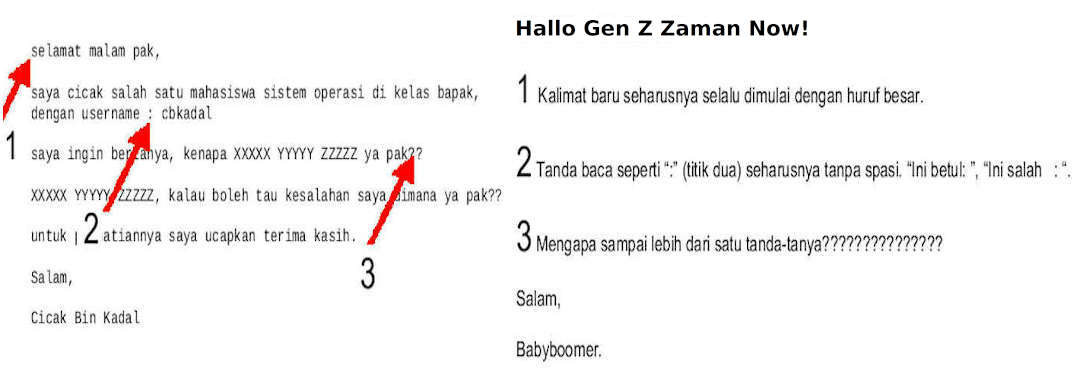
\includegraphics[width=1.01\linewidth]{os-millenial-mail}
\end{figure}
\end{frame}

% XXXXXXXXXXXXXXXXXXXXXXXXXXXXXXXXXXXXXXXXXXXXXXXXXXXXXXXXXXXXXXXXXXXXXXXXXX
\section{Assessment}
\begin{frame}
\frametitle{Assessment}
\begin{itemize}
\item \textbf{11 Weekly Assignments @ 11.11 points}.
\begin{itemize}
\item Assignments will vary from week to week.
\item The assignment deadline will be by the end of every week. 
See \url{https://os.vlsm.org/\#idx02}.
\item Check your points regularly at \url{https://academic.ui.ac.id/}
\item See also, \url{https://os.vlsm.org/Log/}.
\item \textbf{DO NOT COMPLAIN} weeks after! 
\end{itemize}
\item You need to log your weekly activities!
\begin{itemize}
\item See \url{https://doit.vlsm.org/ETC/logCodes.txt}
\item See \url{https://cbkadal.github.io/os242/TXT/mylog.txt}
\item \textbf{4 SKS} (Units) means 12 hours (720 minutes) per week!
\item The average time allocation for each weekly assignment is 
      425 minutes—only 45\% of the four SKS (units) load.
\item Most of the time (44 \%) will be spent on the weekly assignment.
\end{itemize}
\end{itemize}

\end{frame}

% XXXXXXXXXXXXXXXXXXXXXXXXXXXXXXXXXXXXXXXXXXXXXXXXXXXXXXXXXXXXXXXXXXXXXXXXXX
\section{Average Time Allocation}
\begin{frame}
\frametitle{Average Time Allocation}

\begin{figure}
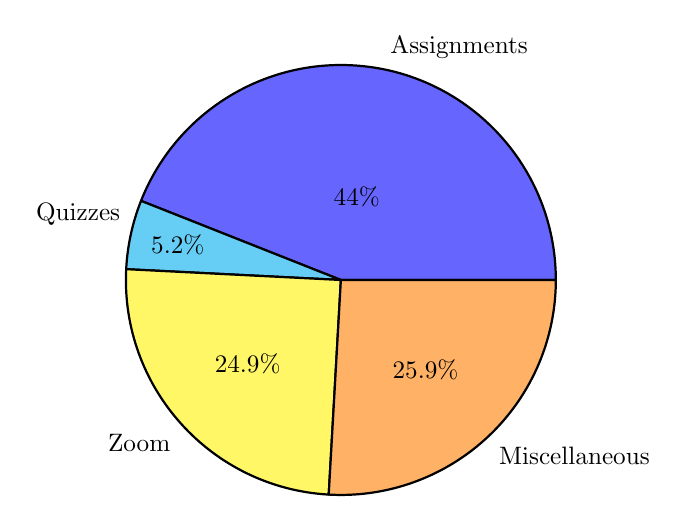
\begin{tikzpicture}[scale=0.91, transform shape]
\pie{44/Assignments,
      5.2/Quizzes,
     24.9/Zoom,
     25.9/Miscellaneous}
\end{tikzpicture}
\caption{Operating Systems classes (2021-2022) student time allocation chart}
\end{figure}

\end{frame}

% XXXXXXXXXXXXXXXXXXXXXXXXXXXXXXXXXXXXXXXXXXXXXXXXXXXXXXXXXXXXXXXXXXXXXXXXXX
\section{NFT: Non-Fungible Tests}
\begin{frame}
\frametitle{NFT: Non-Fungible Tests}
\begin{itemize}

\item Midterm (UTS)
\begin{itemize}
\item The Midterm (UTS) is mandatory \textbf{IF} your SCORE is less than 25.0 before UTS.
      Otherwise, you need to register if you want to take UTS.
\item The UTS result will replace the worst grade of Assignment 00-05, 
      even if the result is less.
\end{itemize}
\item Final Term (UAS)
\begin{itemize}
\item The final term (UAS) is mandatory \textbf{IF} your SCORE is less than 55.0 before UAS.
      Otherwise, you need to register if you want to take UAS.
\item The UAS result will replace the worst grade of Assignments 06-10,
      even if the result is less.
\end{itemize}
\item Both UTS and UAS can only be held offline in an exam room.
\item You can read an A4 size MEMO -- reciprocal -- written in your \textbf{handwriting}.
\item Failure to show up on the day of the exam without reason and evidence will get a score of "0".
\end{itemize}
\end{frame}

% XXXXXXXXXXXXXXXXXXXXXXXXXXXXXXXXXXXXXXXXXXXXXXXXXXXXXXXXXXXXXXXXXXXXXXXXXX
\section{Final Grade}
\begin{frame}
\frametitle{Final Grade (1)}

\begin{itemize}
\item The final grade will be the best 9 out of 11 assignments.
\item \textbf{Two (2) ''spare'' assignments will be more than enough!}
\item In case of emergency, contact your Academic Advisor!
\item C-2C (C minus to C)
\begin{itemize}
\item Up to 5 points, only if:
\begin{itemize}
\item your grade is between 50.00 and 55.00, and
\item you have a ''good'' track record.
\end{itemize}
\end{itemize}

\item Score Range\\[10pt]
\begin{tabular}{l l l l}
\hline
85 - ... = A & 80 - 85 = A- & 75 - 80 = B+ & 70 - 75 = B \\
65 - 70 = B-      & 60 - 65 = C+ & 55 - 60 = C  & 
50 - 55 = D or C\footnote{C-2C: terms and conditions apply --- void where prohibited by law.}  \\
40 - 50 = D  & 30 - 40 = E  & 20 - 30 = \small E & 00 - 20 = \tiny E   \\
\hline \end{tabular}\\[10pt]
\end{itemize}
\end{frame}

% XXXXXXXXXXXXXXXXXXXXXXXXXXXXXXXXXXXXXXXXXXXXXXXXXXXXXXXXXXXXXXXXXXXXXXXXXX
\begin{frame}[fragile]
\frametitle{The eternal recurring chronic problem} 

\textbf{How to avoid receiving emails like the following at the end of the semester after grades have 
        been published?}

\begin{figure}
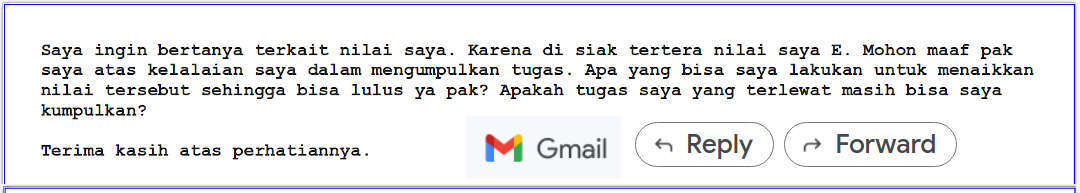
\includegraphics[width=1.01\linewidth]{os-appeal}
\end{figure}

\begin{itemize}
\item Do not ask for any dispensations like a broken computer, circumcision (sunat), cold, competitions
      (including Gemastik), deadline extension, influenza, lame excuses, marriage, mourning,
      power failure, remedial, return to the village (mudik), slow network (lemot), two-semester evaluation, umrah,
      weddings, etc.
\item It also includes: ''It is not my fault but of $\{ X\!: X\ \in\ Lecturer\ \parallel\ Fasilkom\
      \parallel\ UI\ \parallel\ Kampus\ Merdeka\ \parallel\ Immigration\ \parallel\ Foreign\ Embassy\ \parallel\
      else\, \}$.''
\end{itemize}

\end{frame}

% XXXXXXXXXXXXXXXXXXXXXXXXXXXXXXXXXXXXXXXXXXXXXXXXXXXXXXXXXXXXXXXXXXXXXXXXXX
\begin{frame}[fragile]
\frametitle{Grade Examples}

\begin{figure}
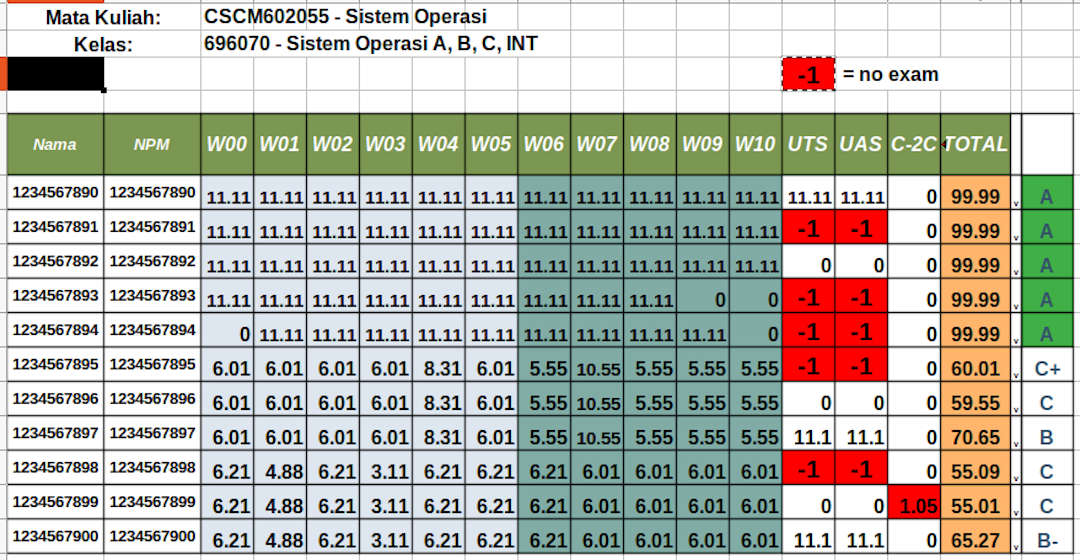
\includegraphics[width=0.94\linewidth]{os-siak}
\end{figure}

\end{frame}

% XXXXXXXXXXXXXXXXXXXXXXXXXXXXXXXXXXXXXXXXXXXXXXXXXXXXXXXXXXXXXXXXXXXXXXXXXX
\section{The Three-Strikes Rule}
\begin{frame}[fragile]
\frametitle{The Three-Strikes Rule}

\begin{figure}
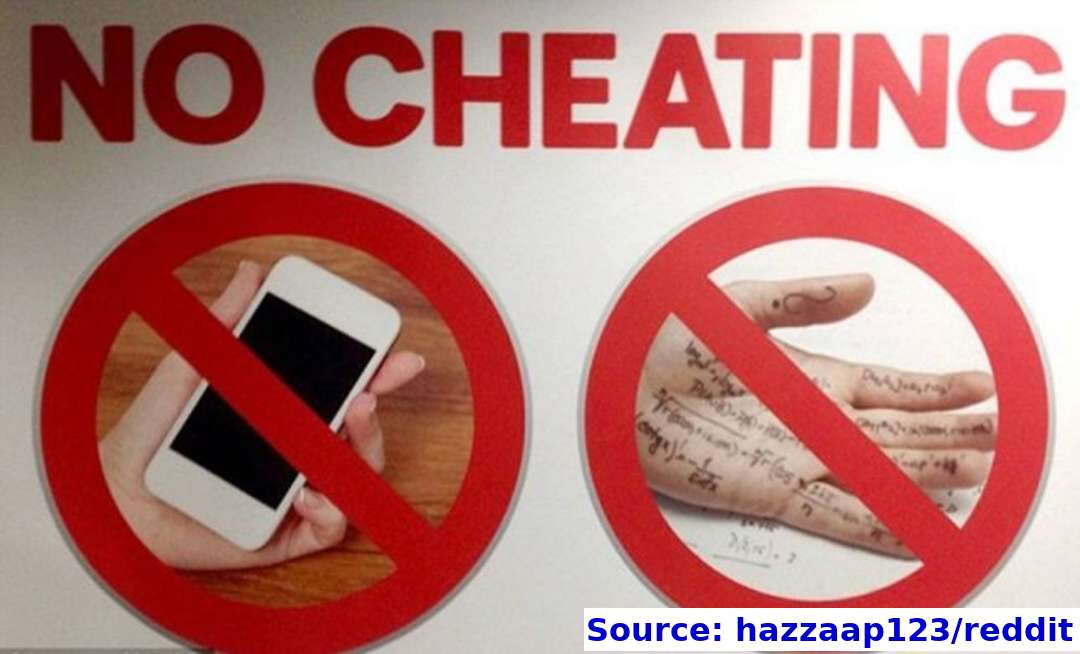
\includegraphics[width=0.30\linewidth]{os-cheating}
\end{figure}

\begin{itemize}
\item All major academic rules violations will be handled directly by the Faculty of Computer Science,
University of Indonesia.
\item ''Accidents'' may happen. There will be warnings for the first two minor violations.
\item Your final grade will be reduced for the third warning.
\item Your final grade will be reduced to "D" for the fourth warning.
\item Five (5) or more warnings will be considered as a significant academic-rules violation.
\end{itemize}

\end{frame}

% XXXXXXXXXXXXXXXXXXXXXXXXXXXXXXXXXXXXXXXXXXXXXXXXXXXXXXXXXXXXXXXXXXXXXXXXXX
\begin{frame}[fragile]
\frametitle{AIN'T DIFFICULT, lah!}
\begin{figure}
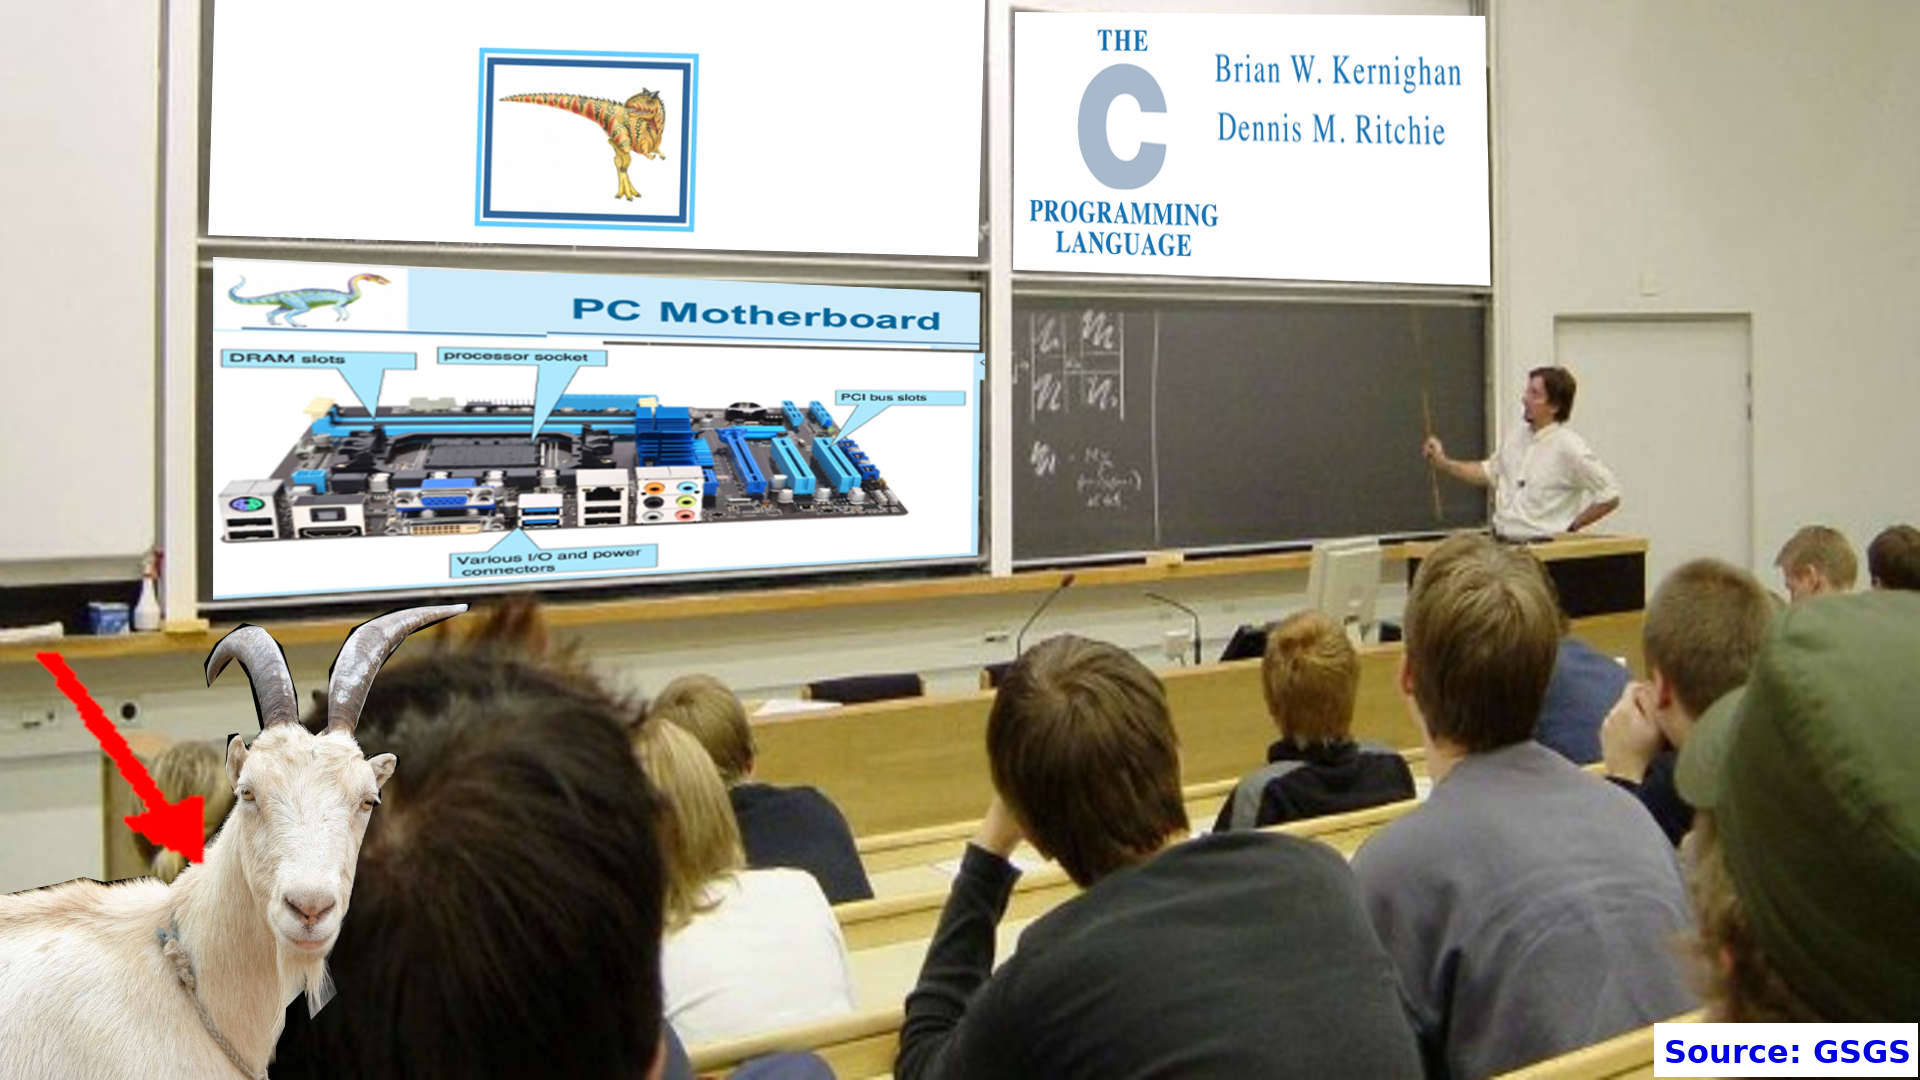
\includegraphics[width=0.79\linewidth]{os-kambing-kuliah-c}
\caption{Even this Goat will get ''C'' at the end of the semester!}
\end{figure}
\end{frame}

% XXXXXXXXXXXXXXXXXXXXXXXXXXXXXXXXXXXXXXXXXXXXXXXXXXXXXXXXXXXXXXXXXXXXXXXXXX
\section{Study From Anywhere?}
\begin{frame}[fragile]
\frametitle{Study From Anywhere?}
\begin{figure}
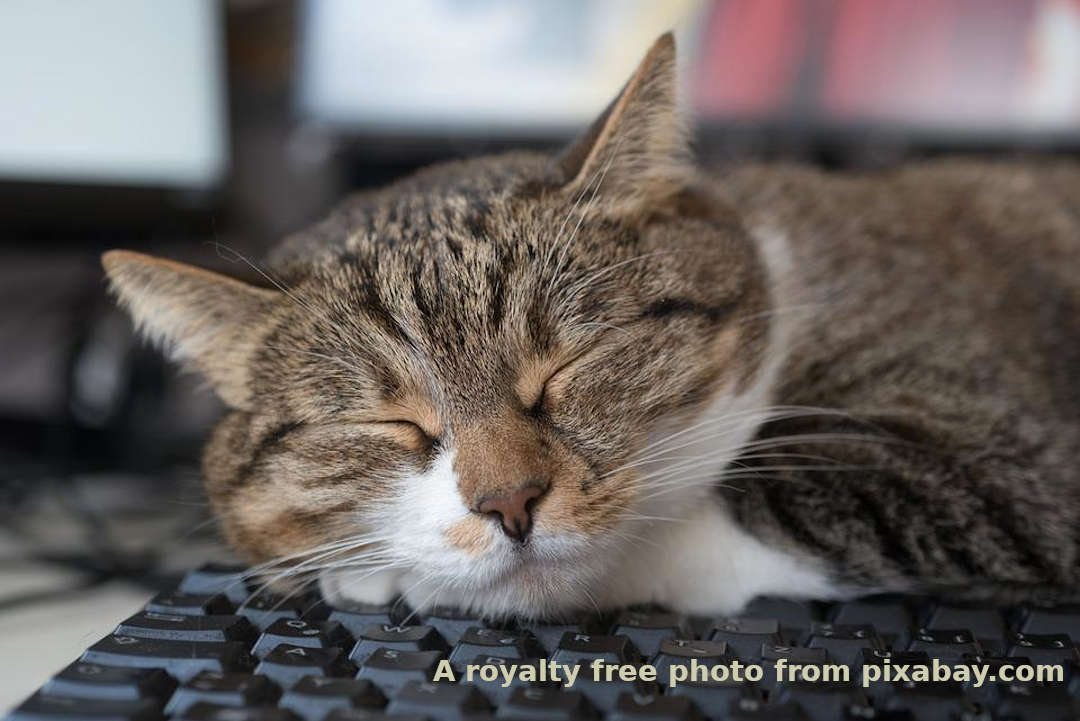
\includegraphics[width=0.64\linewidth]{os-cat}
\caption{Who is on Zoom? What? I don't know! Why? Because! Today, I Don't Give a Darn!}
\end{figure}
\end{frame}

% XXXXXXXXXXXXXXXXXXXXXXXXXXXXXXXXXXXXXXXXXXXXXXXXXXXXXXXXXXXXXXXXXXXXXXXXXX
\begin{frame}[fragile]
\frametitle{Prelude: Daisy Bell -- Bicycle Built for Two}
\begin{tabular}{cc}
\begin{minipage}{45mm}
\vspace{1pt}
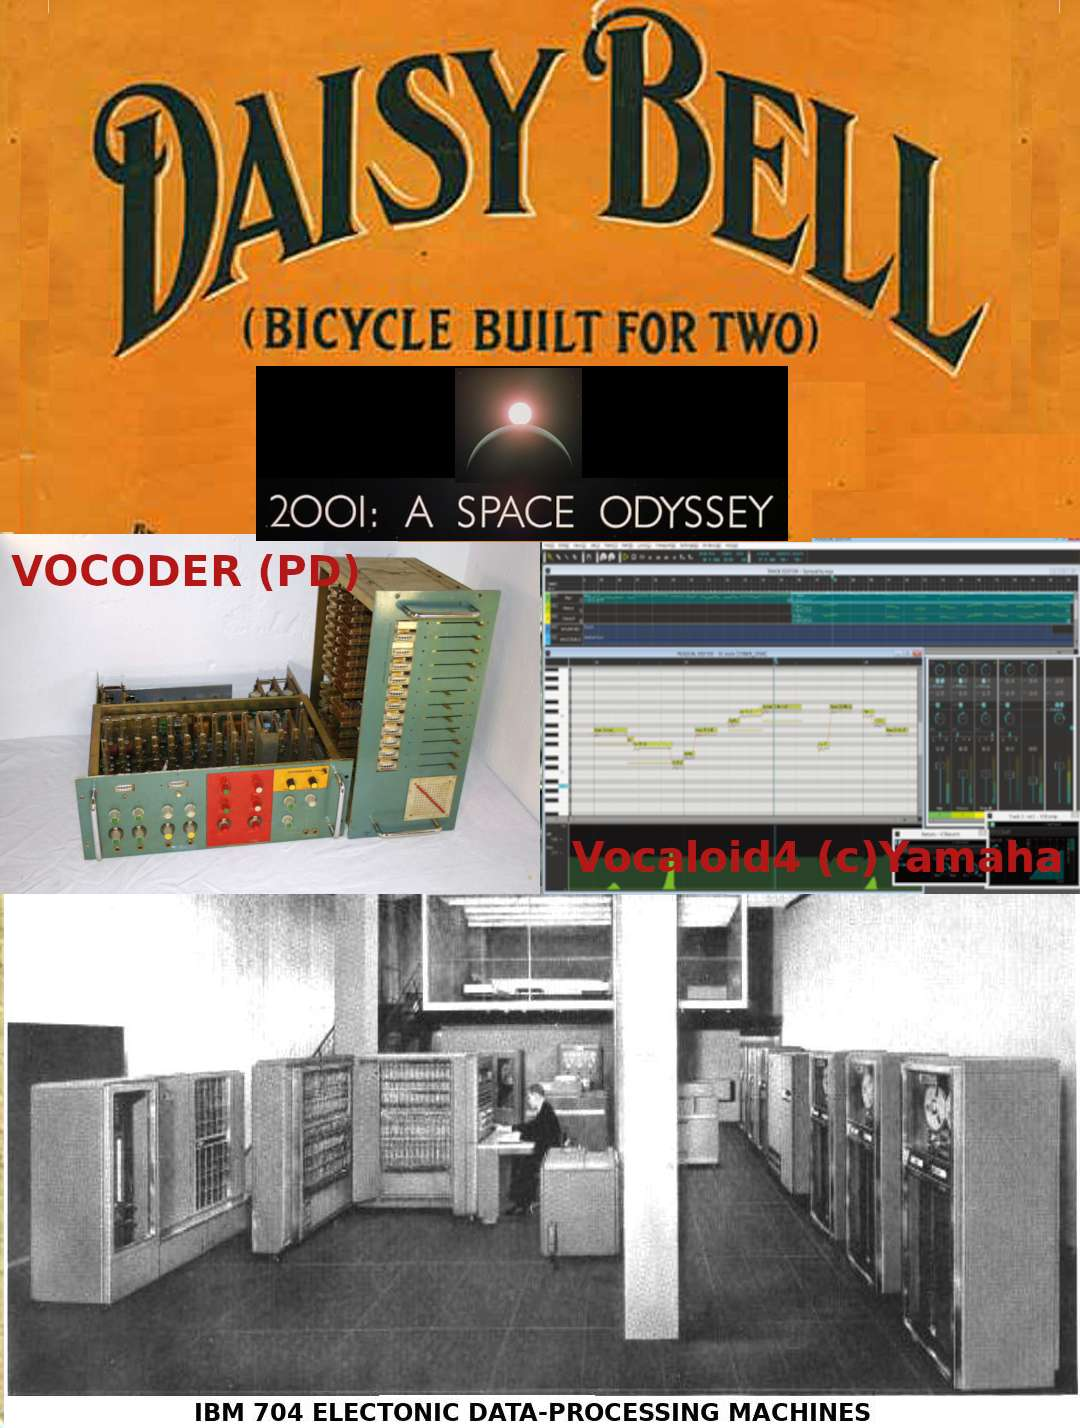
\includegraphics[width=0.89\linewidth]{os-daisybell}
\end{minipage}
&
\begin{minipage}{65mm}
\vspace{1pt}
\begin{verbatim}
Daisy, Daisy,
Give me your answer, do!
I'm half crazy,
All for the love of you!
It won't be a stylish marriage,
I can't afford a carriage,
But you'll look sweet on the seat
Of a bicycle built for two!
\end{verbatim}
\end{minipage}
\\
\end{tabular}
\\[5mm]

YouTube {\footnotesize  (\url{https://youtu.be/TXK_cE9AqAI})}.
A choir (emulation) of 
\href{https://youtu.be/TXK_cE9AqAI?t=68}{VOCODER}
(pre WW2), 
\href{https://youtu.be/TXK_cE9AqAI?t=99}{IBM704}
(1950s) and 
\href{https://youtu.be/TXK_cE9AqAI?t=130}{Vocaloid4}
(2014).
See also the classical movie \href{https://youtu.be/oR\_e9y-bka0}{2001: A Space Odyssey}. 
\end{frame}

% XXXXXXXXXXXXXXXXXXXXXXXXXXXXXXXXXXXXXXXXXXXXXXXXXXXXXXXXXXXXXXXXXXXXXXXXXX
\begin{frame}
\frametitle{IBM 704 at Los Alamos National Laboratory in the 1950s}
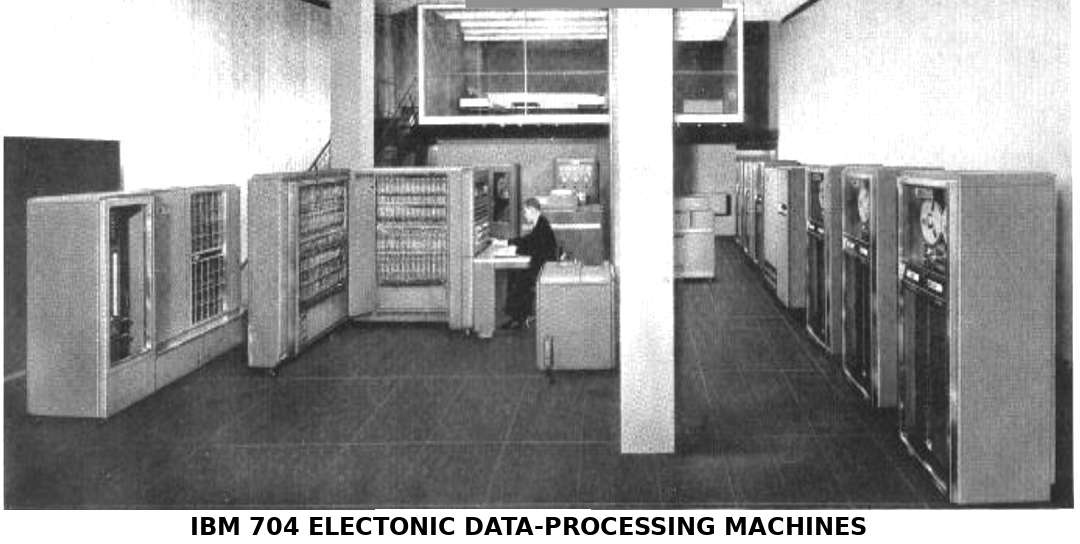
\includegraphics[width=0.75\linewidth]{os-ibm704}

Estimate price (2020 value): USD 8,000,000.

Weight: 8800 kg --- Electricity: ca. 200 kWatt --- 42000 flops --- 
128 kbytes (eq.) core memory --- 64 kbytes (eq.) drum memory --- 3 Mbytes (eq.) Tape Unit.

\end{frame}

% XXXXXXXXXXXXXXXXXXXXXXXXXXXXXXXXXXXXXXXXXXXXXXXXXXXXXXXXXXXXXXXXXXXXXXXXXX
\begin{frame}
\frametitle{Xiaomi 12 Pro -- 12 GB / 256 GB}
\begin{figure}
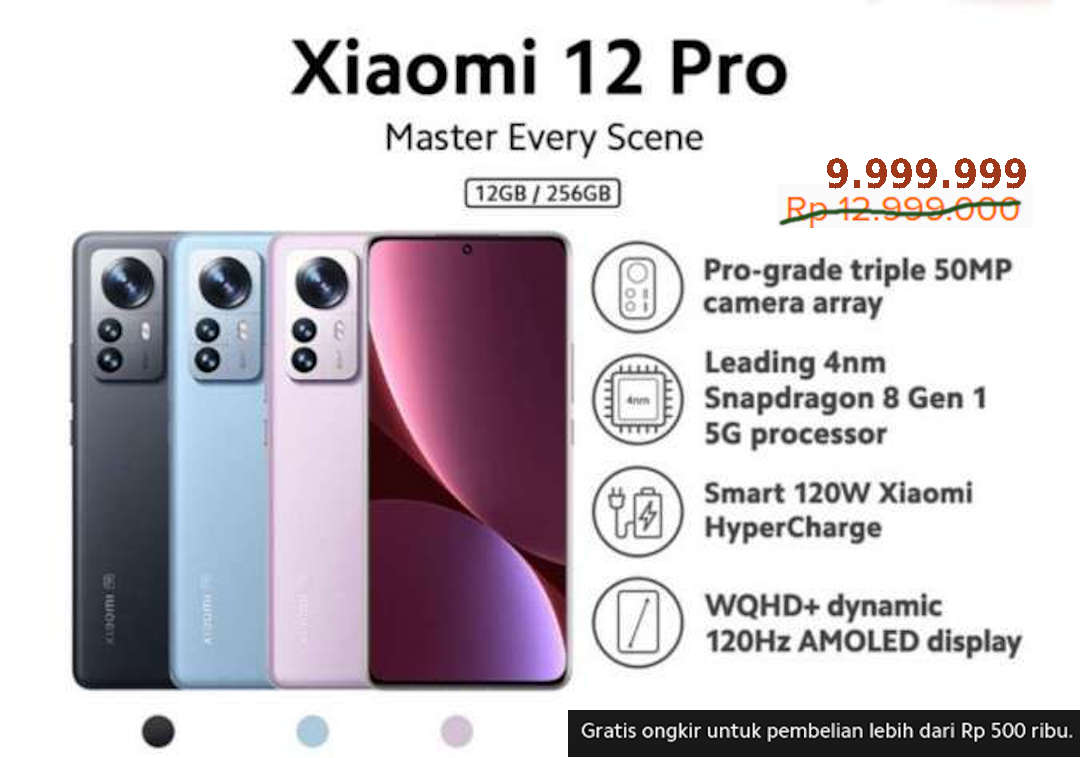
\includegraphics[width=0.63\linewidth]{xiaome12pro}
\caption{Source: Mi Indonesia (2024)}
\end{figure}
\end{frame}

% XXXXXXXXXXXXXXXXXXXXXXXXXXXXXXXXXXXXXXXXXXXXXXXXXXXXXXXXXXXXXXXXXXXXXXX
\section{Miscellaneous}
\begin{frame}[fragile]
\frametitle{Out of Topic/Intermezzo/Segue}
\begin{itemize}
\item Semiconductor Scalling:
\begin{itemize}
\item Process Shrink: $10 \mu{}m$ (1971), $250 nm$ (1996), $10 nm$ (2016), $5 nm$ (2020), $3 nm$ (2022).
\item Smaller Devices means:
\begin{itemize}
\item Less space.
\item Less power consumption.
\item More density.
\end{itemize}
\end{itemize}
\item Indonesia:
\begin{itemize}
\item Fairchild Semiconductor Indonesia.
\item National Semiconductor Indonesia.
\item Minister of Manpower (Menteri Tenaga Kerja) 1983–1988.
\end{itemize}
\item Technology:
\begin{itemize}
\item SoC: System on a Chip.
\item SiP: System in a Package.
\item Fab/Foundry: Taiwan Semiconductor Manufacturing Company (TSMC), Ltd.
\begin{itemize}
\item Have No Fab? It is OK! E.g., Marvell Technology, Inc (1995).
\end{itemize}
\item Lithography: ASML Holding, N.V: Advanced Semiconductor Materials Lithography.
\item Optics: Carl Zeiss SMT GmbH (This is NOT Optik Seis, Duh :).
\end{itemize}
\end{itemize}
\end{frame}

% XXXXXXXXXXXXXXXXXXXXXXXXXXXXXXXXXXXXXXXXXXXXXXXXXXXXXXXXXXXXXXXXXXXXXXX
\begin{frame}[fragile]
\frametitle{TSMC Logic Nodes}
\begin{figure}
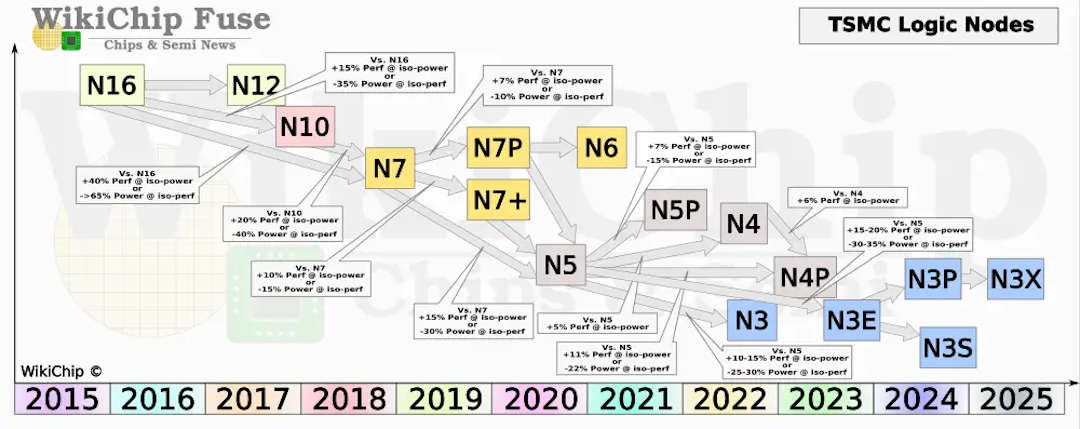
\includegraphics[width=0.95\linewidth]{tsmc_logic_node}
\caption{Source: 
  \href{https://fuse.wikichip.org/wp-content/uploads/2022/09/wikichip_tsmc_logic_node_q2_2022-2.png}{WikiChip}}
\end{figure}
\end{frame}

% XXXXXXXXXXXXXXXXXXXXXXXXXXXXXXXXXXXXXXXXXXXXXXXXXXXXXXXXXXXXXXXXXXXXXXX
\begin{frame}[fragile]
\frametitle{The Computing Diciplines}
\begin{figure}
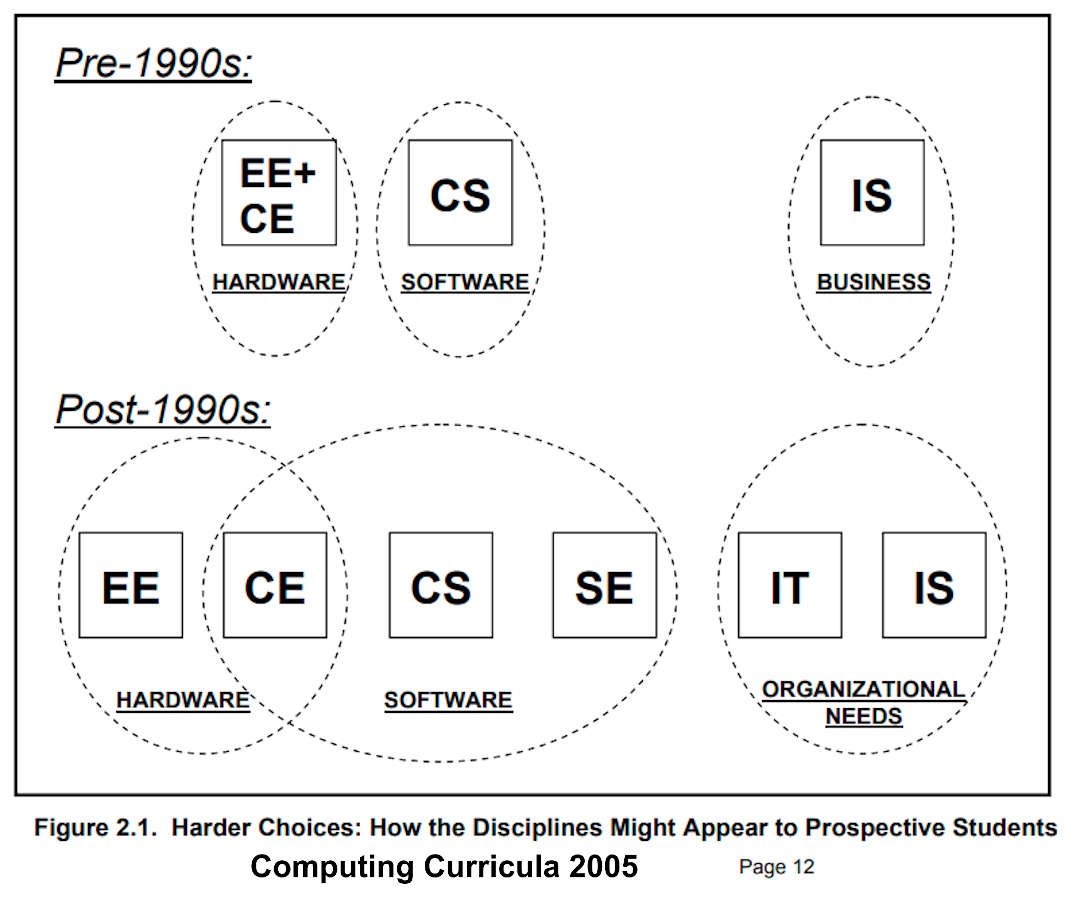
\includegraphics[width=0.59\linewidth]{pic-cc2005}
\caption{The Computing Diciplines}
\end{figure}
\end{frame}

% XXXXXXXXXXXXXXXXXXXXXXXXXXXXXXXXXXXXXXXXXXXXXXXXXXXXXXXXXXXXXXXXXXXXXXXXXX
\begin{frame}[fragile]
\frametitle{Lessons from the Development of the Boeing 787 Dreamliner}
\begin{itemize}
\item 1997: Boeing acquired the nearly bankrupt  McDonnell Douglas.
\begin{itemize}
\item Result: "Boeing honorable name" with "McDonnell Douglas Greedy Culture."
\end{itemize}
\item 2003: Boeing announced the Boeing 787 Dreamliner project.
\item 2007: An "empty skeleton" prototype was rolled out on schedule. Many fuselage parts were temporarily attached.
\begin{itemize}
\item Result: as expected, its stock price rose sharply.
\end{itemize}
\item 2009: maiden flight after multiple delays.
\begin{itemize}
\item Problem: Boeing and its partners have had no experience with many new technologies.
\end{itemize}
\item 2011: Enter into service, but the problems did not go away.
\begin{itemize}
\item Result: The budget increased from US\$ 5billion to more than US\$ 30billion.
\end{itemize}
\item 2018: Problems did not go away but were overshadowed by the Boeing 737 MAX problems.
\item Lesson learned?
\end{itemize}
\end{frame}

% XXXXXXXXXXXXXXXXXXXXXXXXXXXXXXXXXXXXXXXXXXXXXXXXXXXXXXXXXXXXXXXXXXXXXXXXXX
\section{LFS: Linux From Scratch}
\begin{frame}
\frametitle{LFS: Linux From Scratch (Week 00 --- Week 10)}
\begin{itemize}
\item \href{https://youtu.be/jEoM3qan9Gs}{THIS IS HOW WE DOIT!}
\item \url{http://www.linuxfromscratch.org/lfs/view/stable/}
\item To build a GNU/Linux system from scratch (source code).
\item To learn a GNU/Linux system inside out.
\item To use a Virtual Machine.
\item A Chicken and Egg dependency problem:
\begin{itemize}
\item It would be best if you had the tools to build an Operating System.
\item You need an Operating System to build tools.
\item To build a cross-toolchain (compiler and its libraries).
\item To build cross utilities using the cross-toolchain.
\item To build an Operating System in a chroot environment.
\item To do iterations (if necessary).
\end{itemize}
\item How deep would you like to know of a ''real'' Operating System?
\item Whatever, however, from Week 00 to Week 10!
\item \textbf{YOU} decide!
\end{itemize}
\end{frame}

% XXXXXXXXXXXXXXXXXXXXXXXXXXXXXXXXXXXXXXXXXXXXXXXXXXXXXXXXXXXXXXXXXXXXXXXXXX
\section{What defines an Operating System? (The Three Layers Model)}
\begin{frame}
\frametitle{What defines an Operating System? (The Three Layers Model)}
\begin{multicols}{2}
\begin{table}
\scalebox{0.8}{%
\begin{tabular}{| c |}
\hline \\ [1pt]
Business Goal \\
\vline \\ [1pt]
Application \\
\vline \\ [1pt]
\hline
OS API \\
\vline \\ [1pt]
OS Managers and Utilities \\
\vline \\ [1pt]
OS Drivers \\
\hline
\vline \\ [1pt]
(Hypervisor) \\
\vline \\ [1pt]
Hardware \\ [1pt]
\hline
\end{tabular}}
\end{table}
  \vfill \null
\columnbreak
  \begin{itemize}
    \item The Three Layers Model
  \begin{itemize}
    \item An Operating System is between your Application and your Hardware (or Hypervisor).
  \begin{itemize}
    \item OS API: Application Programming Interface
    \item OS Resources Managers and Utilities: Process, Scheduler, Dispatcher, 
             (Virtual) Memory, Disk, I/O, Network, Security, Protection, etc.
    \item OS Device Drivers: controls devices
  \end{itemize}
    \item Remember that your future "\textbf{Business Goal}" may not directly relate to an Operating System at all!
  \end{itemize}
  \end{itemize}
  \vfill \null
\end{multicols}
\end{frame}

% XXXXXXXXXXXXXXXXXXXXXXXXXXXXXXXXXXXXXXXXXXXXXXXXXXXXXXXXXXXXXXXXXXXXXXXXXX
\section{OSC10 (Silberschatz) Chapter 1 and 2}
\begin{frame}
\frametitle{OSC10 (Silberschatz) Chapter 1 and 2}
\begin{multicols}{2}
  \begin{itemize}
  \item OSC10 Chapter 1
  \begin{itemize}
  \item What Operating Systems Do
  \item Computer-System Organization
  \item Computer-System Architecture
  \item Operating-System Operations
  \item Resource Management
  \item Security and Protection
  \item Virtualization
  \item Distributed Systems
  \item Kernel Data Structures
  \item Computing Environments
  \item Free/Libre and Open-Source Operating Systems
  \end{itemize}
  \end{itemize}
  \vfill \null
\columnbreak
  \begin{itemize}
  \item OSC10 Chapter 2
  \begin{itemize}
  \item Operating System Services
  \item User and Operating System-Interface
  \item System Calls
  \item System Services
  \item Linkers and Loaders
  \item Why Applications are Operating System Specific
  \item Operating-System Design and Implementation
  \item Operating System Structure
  \item Building and Booting an Operating System
  \item Operating System Debugging
  \end{itemize}
  \end{itemize}
  \vfill \null
\end{multicols}
\end{frame}

% XXXXXXXXXXXXXXXXXXXXXXXXXXXXXXXXXXXXXXXXXXXXXXXXXXXXXXXXXXXXXXXXXXXXXXXXXX
\begin{frame}
\frametitle{Remember Computer Organization (POK/DDAK)?}
\begin{itemize}
\item You should understand:
\begin{itemize}
\item von Neumann Model.
\item Buses, Bridges, Transfer Rate, Clock.
\item Memory: DDR, DDR-2, DDR-3, DDR-3+ ...
\item Cache, Buffer, Spool, \& Pipelining.
\item Direct Memory Access (DMA).
\item Port \& Memory Mapped I/O.
\item CPU: (privilege/kernel/supervisor mode) vs. (user mode).
\item Physical (Hardware) Limitation.
\item Priority: Read vs. Write.
\item Interrupts: Polling \& Vectored.
\item Multiprocessors: Symmetric vs. Asymmetric.
\item Multicore \& Multithreading.
\item Clustered Systems.
\item Numbers: base 2, base 8, base 10, base 16.
\begin{itemize}
\item Base 2: $110010101010_2$
\item Base 8: $01234567_8\ =\ 000\ 001\ 010\ 011\ 100\ 101\ 110\ 111_2$
\item Base 10: $012\ 345\ 679$
\item Base 16: $9AB\ CDEF_{16}\ =\ 1001\ 1010\ 1011\ \ 1100\ 1101\ 1110\ 1111_2$
\end{itemize}
\end{itemize}
\end{itemize}
\end{frame}

% XXXXXXXXXXXXXXXXXXXXXXXXXXXXXXXXXXXXXXXXXXXXXXXXXXXXXXXXXXXXXXXXXXXXXXXXXX
\begin{frame}
\frametitle{Physics 101: Signal Length (E.g. 3 GHz)}
\begin{figure}
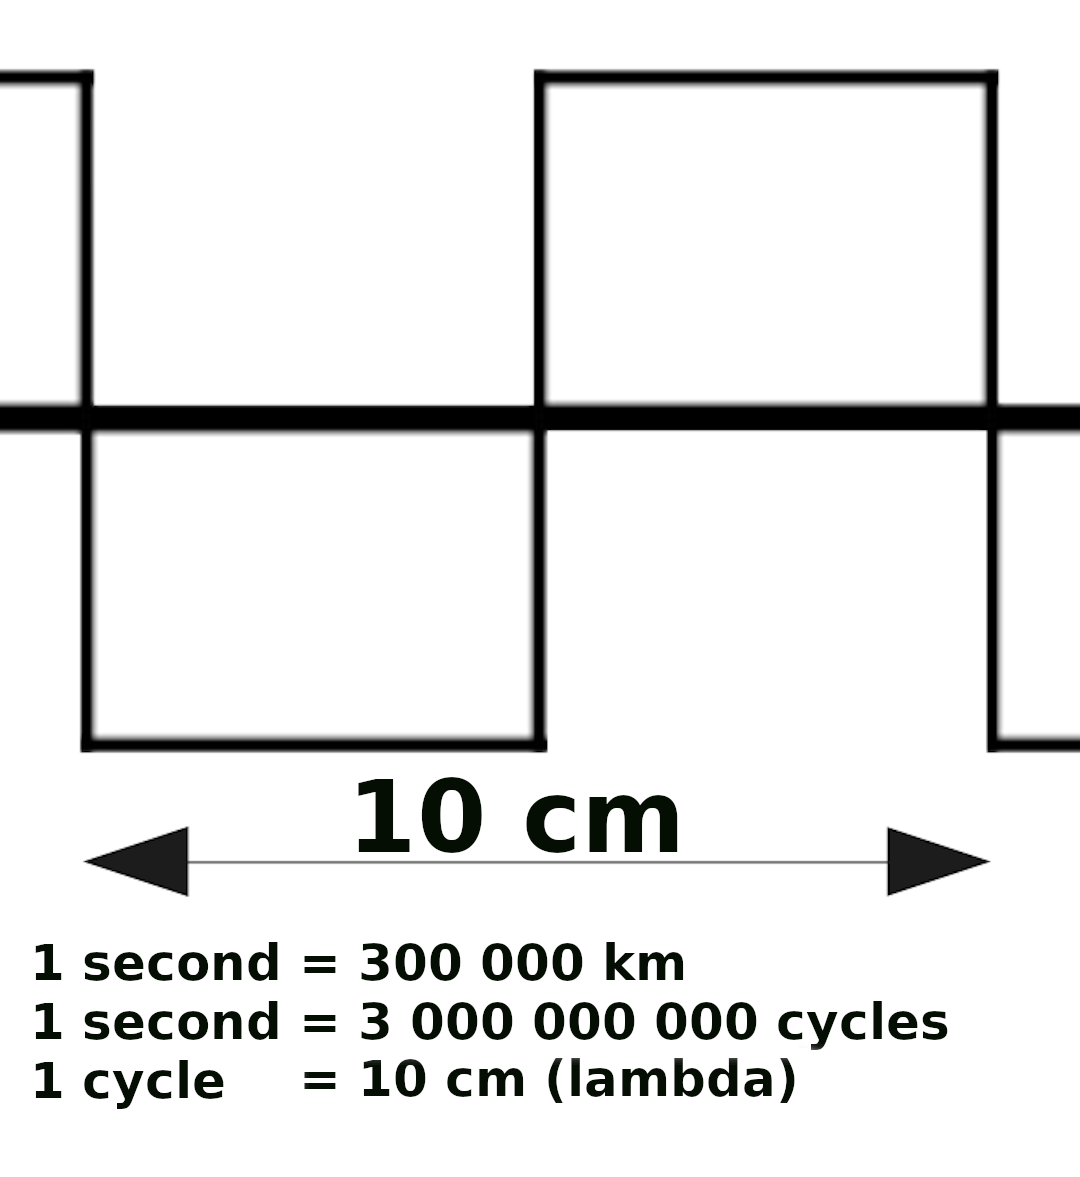
\includegraphics[width=0.40\linewidth]{os-wave3}
\caption{What is the length of a 3 GHz signal?}
\end{figure}
\end{frame}

% XXXXXXXXXXXXXXXXXXXXXXXXXXXXXXXXXXXXXXXXXXXXXXXXXXXXXXXXXXXXXXXXXXXXXXXXXX
\begin{frame}
\frametitle{Physics 101: Safe Distance for 3 GHz}
\begin{figure}
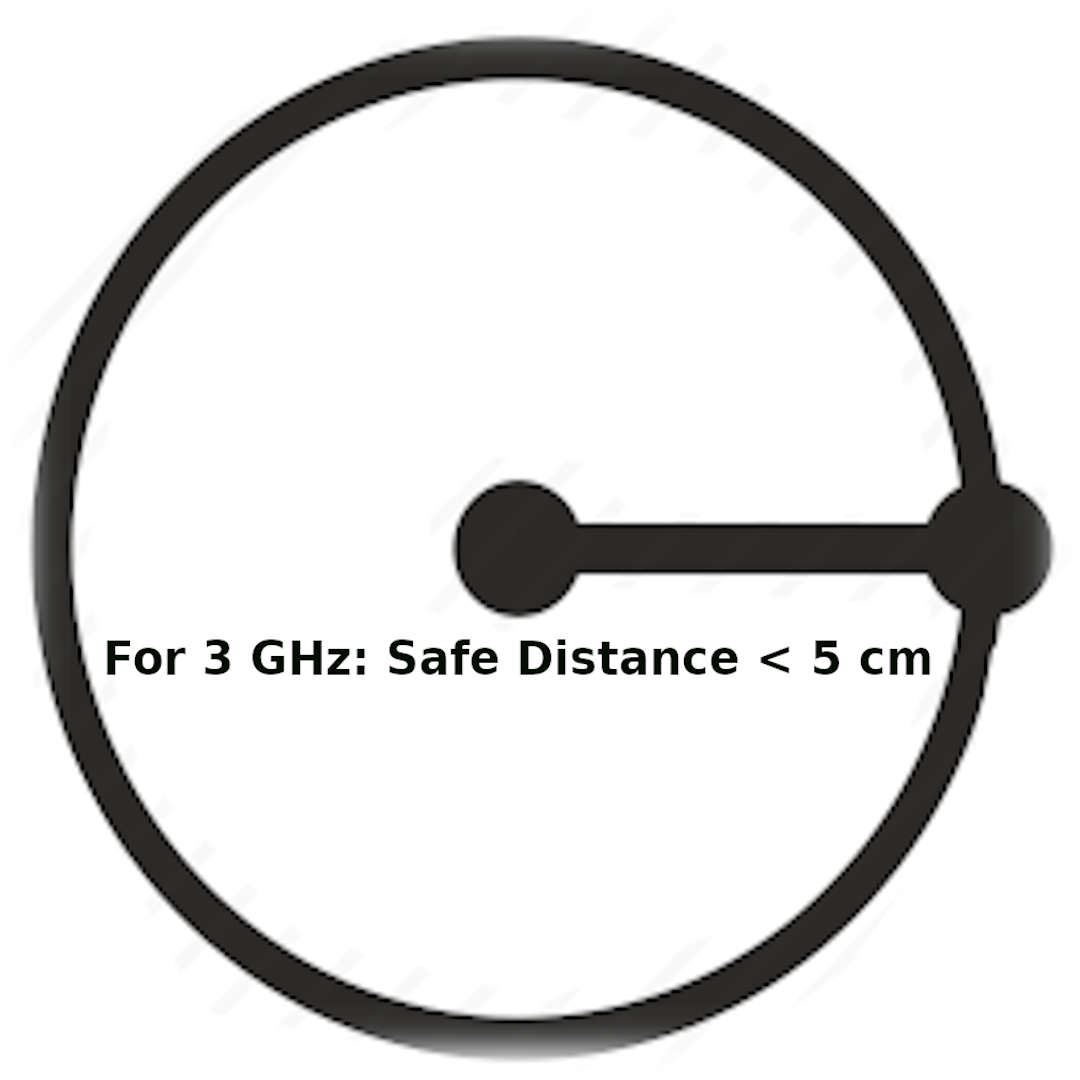
\includegraphics[width=0.45\linewidth]{os-circle}
\caption{Safe Distance}
\end{figure}
\end{frame}

% XXXXXXXXXXXXXXXXXXXXXXXXXXXXXXXXXXXXXXXXXXXXXXXXXXXXXXXXXXXXXXXXXXXXXXXXXX
\begin{frame}
\frametitle{Physics 101: Serial vs. Parallel Transmission}
\begin{multicols}{2}
  \begin{itemize}
    \item Serial Transmission
  \begin{itemize}
    \item Longer Distance
    \item Easy to implement
  \end{itemize}
  \end{itemize}
  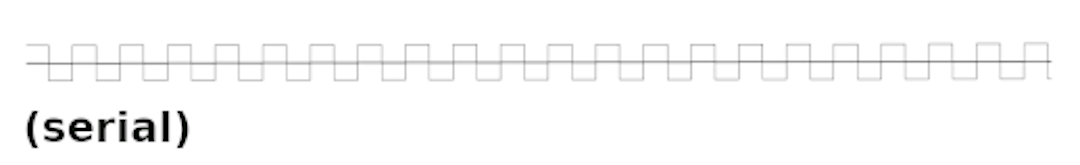
\includegraphics[width=0.99\linewidth]{os-wave4a}
  \vfill \null
\columnbreak
  \begin{itemize}
    \item Parallel Transmission
  \begin{itemize}
    \item Faster
    \item Not easy to implement
  \end{itemize}
  \end{itemize}
  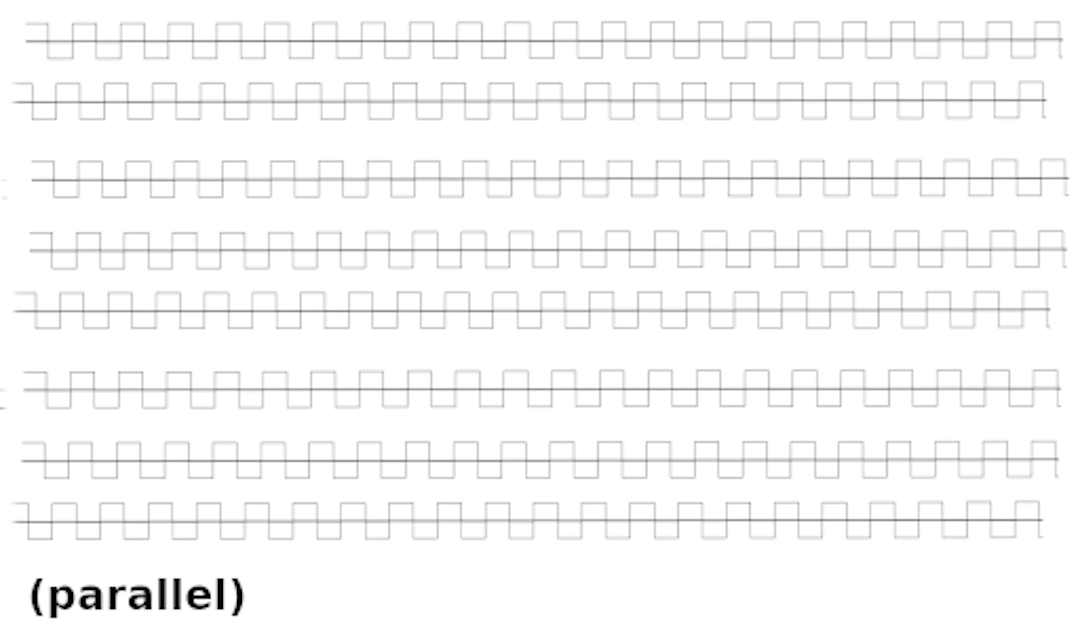
\includegraphics[width=0.99\linewidth]{os-wave4b}
  \vfill \null
\end{multicols}
\end{frame}

% XXXXXXXXXXXXXXXXXXXXXXXXXXXXXXXXXXXXXXXXXXXXXXXXXXXXXXXXXXXXXXXXXXXXXXXXXX
\begin{frame}
\frametitle{Transmission Rate (E.g. \textbf{BUS}: 64 bit/133 MHz)}
\begin{figure}
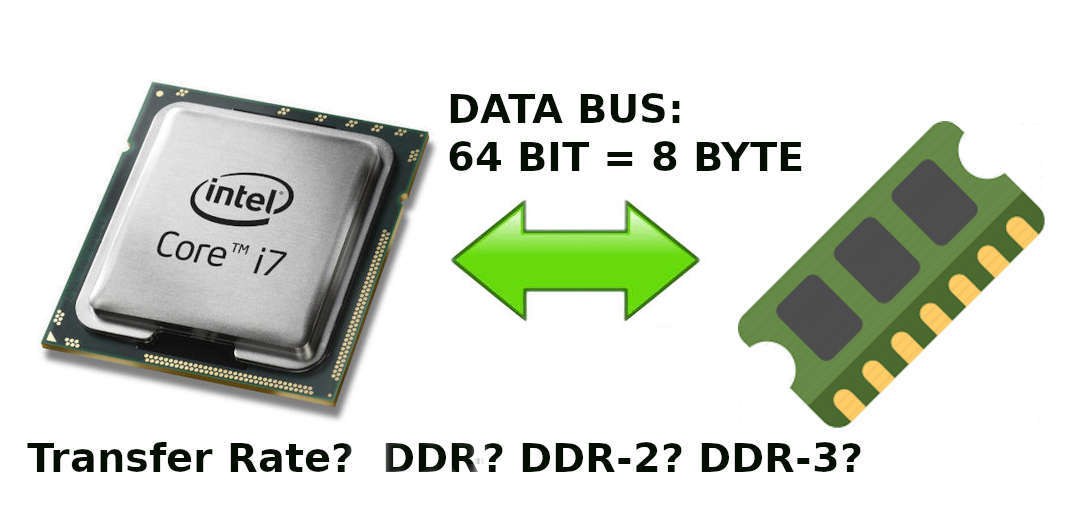
\includegraphics[width=0.40\linewidth]{os-transfer-rate}
\end{figure}
\begin{itemize}
\item E.g. \textbf{BUS}: 64 bit, \textbf{Clock}: 133 MHz
\begin{itemize}
\item SDRAM (Synchronous Dynamic RAM): 1 transmission/cycle.\\
\textbf{Transfer Rate} = \texttt{64/8 byte x 133M x 1 = 1064 Mbyte/s}.
\item DDR (Double Data Rate): 2 transmission/cycle.\\
\textbf{Transfer Rate} = \texttt{64/8 byte x 133M x 2 = 2128 Mbyte/s}.
\item DDR-2 (Double Data Rate 2): 4 transmission/cycle.\\
\textbf{Transfer Rate} = \texttt{64/8 byte x 133M x 4 = 4256 Mbyte/s}.
\item DDR-3 (Double Data Rate 3): 8 transmission per cycle.\\
\textbf{Transfer Rate} = \texttt{64/8 byte x 133M x 8 = 8512 Mbyte/s}.
\item DDR-3+ = DDR-3 with a better clock rate, lower voltage, and greater capacity.
\end{itemize}
\end{itemize}
\end{frame}

% XXXXXXXXXXXXXXXXXXXXXXXXXXXXXXXXXXXXXXXXXXXXXXXXXXXXXXXXXXXXXXXXXXXXXXXXXX
\begin{frame}
\frametitle{CPU: SuperVisor Mode}
\begin{figure}
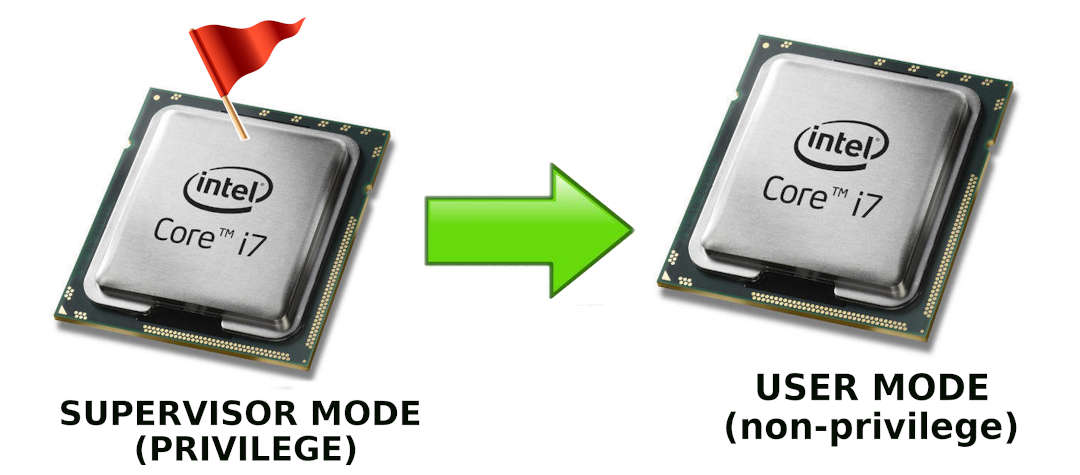
\includegraphics[width=0.50\linewidth]{os-super2user}
\caption{SuperVisor (Privilege) Mode to User Mode}
\end{figure}
\begin{itemize}
\item SuperVisor Mode
\begin{itemize}
\item A.k.a. Kernel Mode, Privilege Mode.
\item Initial STATE (Mode) of a CPU (Power On).
\item STATE (Mode) after Interrupt.
\item All operations are allowed, including to switch to User Mode!
\end{itemize}
\end{itemize}
\end{frame}

% XXXXXXXXXXXXXXXXXXXXXXXXXXXXXXXXXXXXXXXXXXXXXXXXXXXXXXXXXXXXXXXXXXXXXXXXXX
\begin{frame}
\frametitle{CPU: User Mode}
\begin{figure}
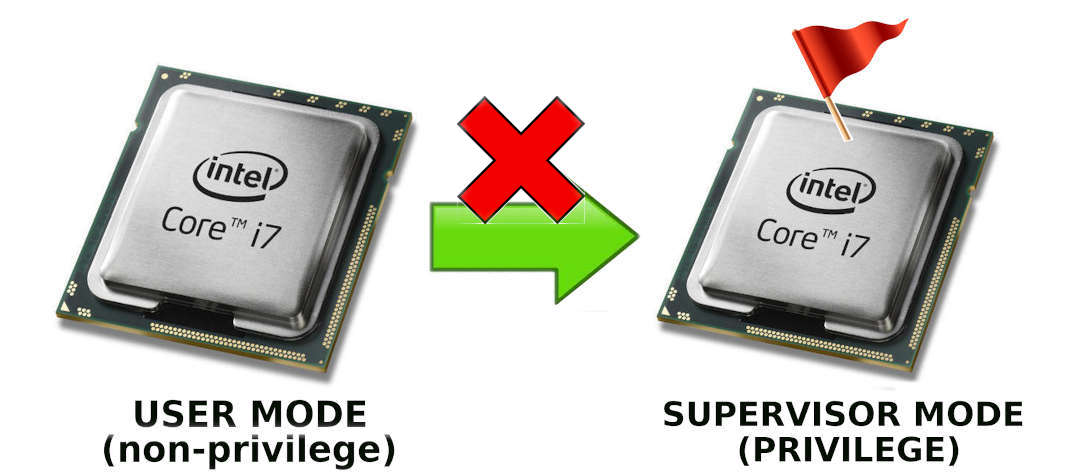
\includegraphics[width=0.50\linewidth]{os-user2super}
\caption{User Mode to SuperVisor (Privilege)}
\end{figure}
\begin{itemize}
\item User Mode
\begin{itemize}
\item It is not allowed to switch back to SuperVisor Mode.
\item It is not allowed to access I/O directly.
\item It is not allowed to modify the Interrupt Vector.
\item It is allowed to request Interrupt.
\end{itemize}
\end{itemize}
\end{frame}

% XXXXXXXXXXXXXXXXXXXXXXXXXXXXXXXXXXXXXXXXXXXXXXXXXXXXXXXXXXXXXXXXXXXXXXXXXX
\begin{frame}
\frametitle{Can you read a Block Diagram?}
\begin{figure}
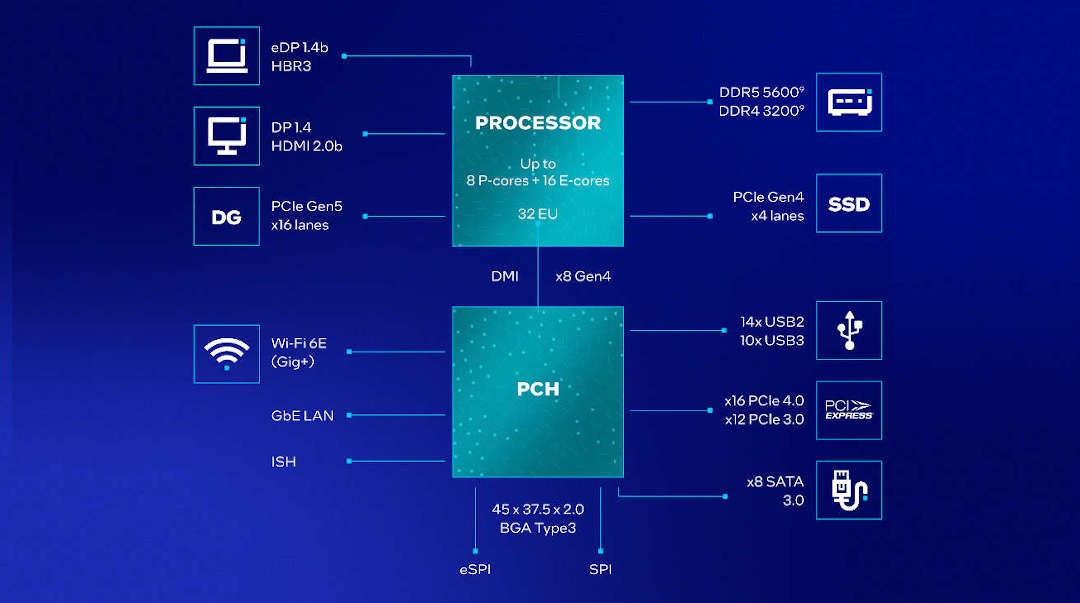
\includegraphics[width=0.79\linewidth]{intel-chipset}
\caption{Block Diagram}
\end{figure}
\end{frame}

% XXXXXXXXXXXXXXXXXXXXXXXXXXXXXXXXXXXXXXXXXXXXXXXXXXXXXXXXXXXXXXXXXXXXXXXXXX
\begin{frame}
\frametitle{Block Diagram}
\begin{itemize}
  \item eDP: Embedded DisplayPort, for internal displays.
  \item DDI: Digital Display Interface
\begin{itemize}
  \item DP: Display Port
  \item HDMI: High-Definition Multimedia Interface
\end{itemize}
  \item DMI: Direct Media Interface
  \item PCIe: Peripheral Component Interconnect express
  \item eSPI: Enhanced Serial Peripheral Interface
  \item SPI: Serial Peripheral Interface
  \item SMBus: System Management Bus
  \item HD Audio: High Definition Audio
  \item USB: Universal Serial Bus
\end{itemize}
\end{frame}

% XXXXXXXXXXXXXXXXXXXXXXXXXXXXXXXXXXXXXXXXXXXXXXXXXXXXXXXXXXXXXXXXXXXXXXXXXX
\begin{frame}
\frametitle{What is an APIC?!}
\begin{figure}
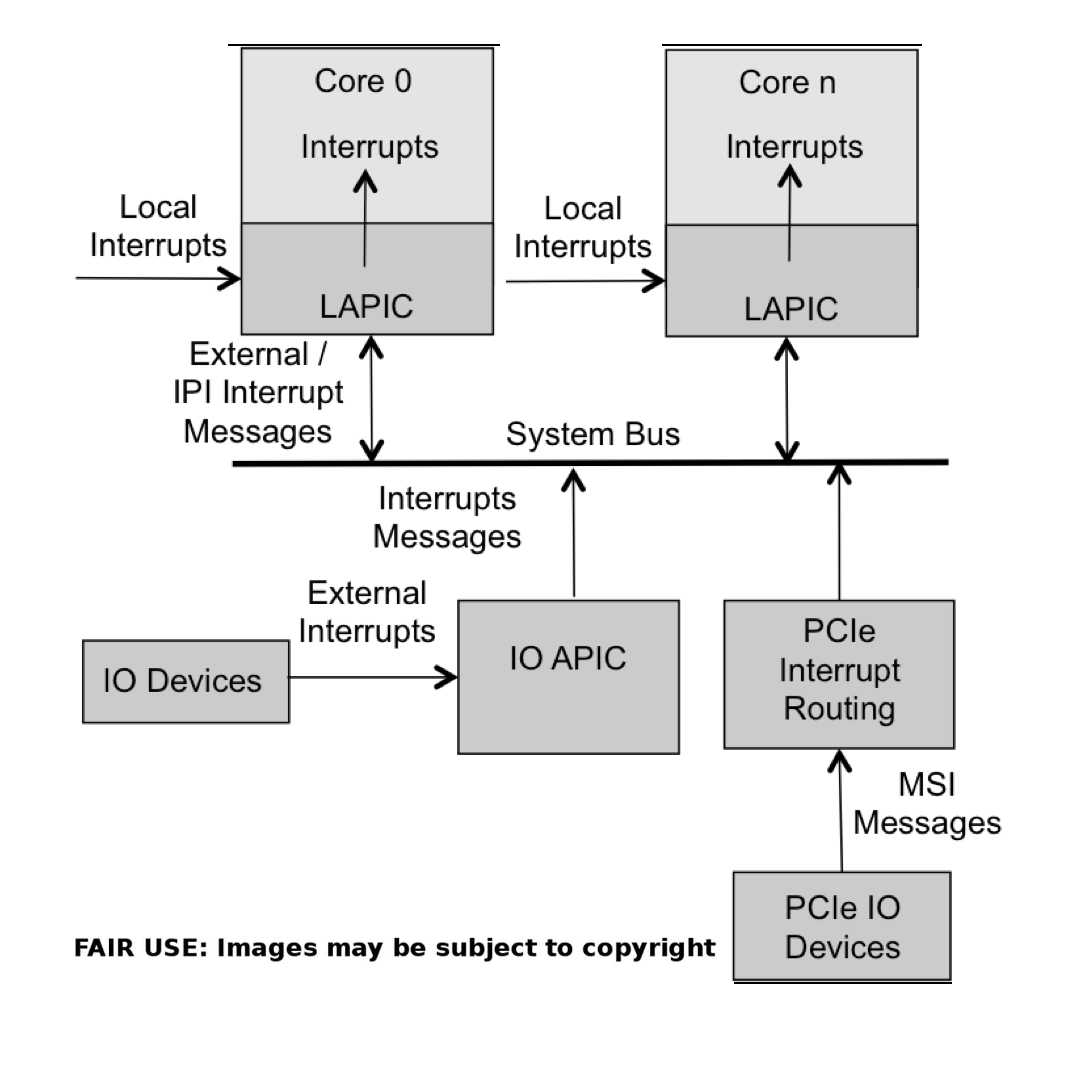
\includegraphics[width=0.44\linewidth]{os00-xapic}
\caption{APIC (Advanced Programmable Interrupt Controller)}
\end{figure}
\end{frame}

% XXXXXXXXXXXXXXXXXXXXXXXXXXXXXXXXXXXXXXXXXXXXXXXXXXXXXXXXXXXXXXXXXXXXXXXXXX
\begin{frame}
\frametitle{And, what is ''Interrupt Handling''?}
\begin{figure}
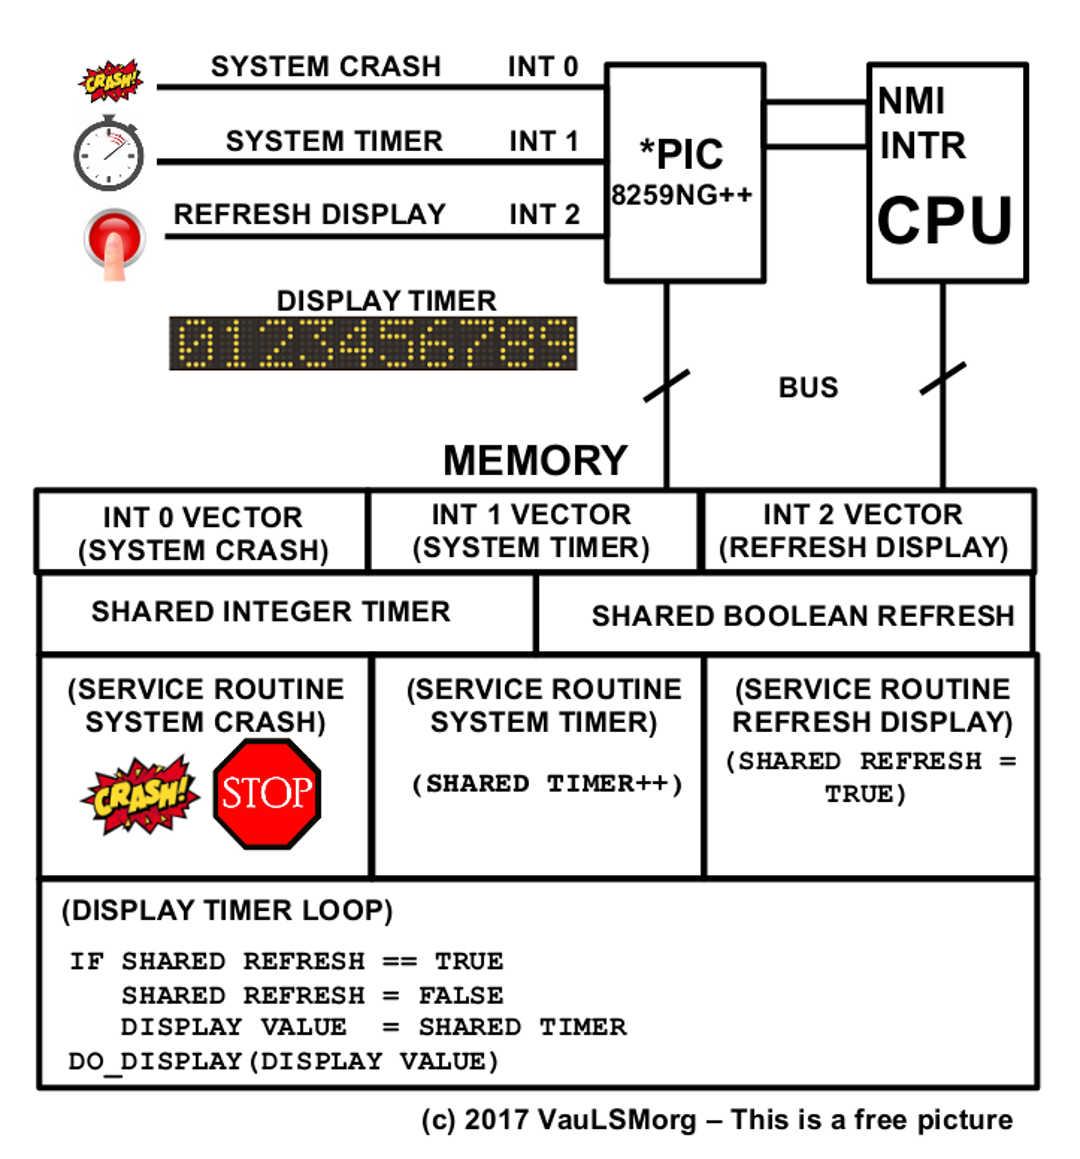
\includegraphics[width=0.40\linewidth]{os00-int-protection}
\caption{Interrupt Handling with PIC (Programmable Interrupt Controller)}
\end{figure}
\end{frame}

% XXXXXXXXXXXXXXXXXXXXXXXXXXXXXXXXXXXXXXXXXXXXXXXXXXXXXXXXXXXXXXXXXXXXXXXXXX
\begin{frame}
\frametitle{The Operating System Managers}
\begin{itemize}
\item Process Manager: 
\begin{itemize}
\item Creating/Deleting; Suspending/Resuming; Synchronization; Communication; Scheduling
\end{itemize}
\item Memory Manager:
\begin{itemize}
\item Tracking; Move In/Move Out; Allocating/Deallocating.
\end{itemize}
\item Storage/File System Manager:
\begin{itemize}
\item Create/Delete; Open/Close; Read/Write.
\end{itemize}
\item Mass Storage Manager:
\begin{itemize}
\item Scheduling; Allocating; Free Space.
\end{itemize}
\item I/O Manager:
\begin{itemize}
\item Buffering; Caching; Spooling.
\item Interfacing (driving).
\end{itemize}
\item Protecting \& Security Manager:
\begin{itemize}
\item Protecting.
\item Security.
\end{itemize}
\end{itemize}
\end{frame}

% XXXXXXXXXXXXXXXXXXXXXXXXXXXXXXXXXXXXXXXXXXXXXXXXXXXXXXXXXXXXXXXXXXXXXXXXXX
\begin{frame}
\frametitle{Any idea what these following terms mean?!}
\begin{itemize}
\item Scripting: bash, regex, sed, awk
\item Security and Protection
\item File System
\item Data Structure in a (logical) Memory
\item Virtual Memory
\item Concurrency
\item Synchronization
\item Mass Storage
\item UEFI, GRUB, and systemd
\item I/O
\item I/O Programming
\end{itemize}
\end{frame}

% XXXXXXXXXXXXXXXXXXXXXXXXXXXXXXXXXXXXXXXXXXXXXXXXXXXXXXXXXXXXXXXXXXXXXXXXXX
\begin{frame}
\frametitle{Week 00: QUIZ Example \#1 (from OSC2e)}
\begin{multicols}{2}

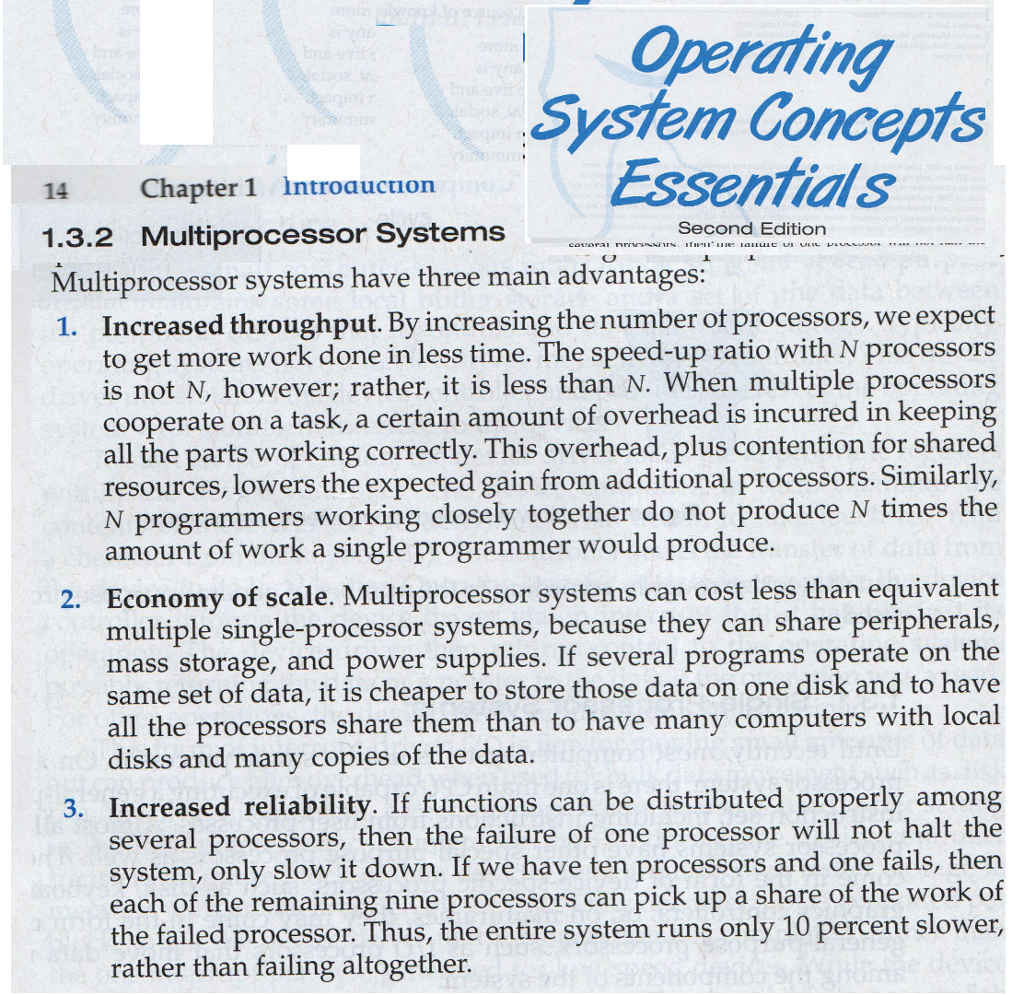
\includegraphics[width=0.97\linewidth]{os00-osc2e}

\columnbreak
  \null \vfill 

  \textbf{True or False?}

  The advantages of a multiprocessor system include: 
  increased throughput, economy of scale, and increased reliability.

  {\footnotesize (from MidTerm 2016)}
  \vfill \null
\end{multicols}
\end{frame}

% XXXXXXXXXXXXXXXXXXXXXXXXXXXXXXXXXXXXXXXXXXXXXXXXXXXXXXXXXXXXXXXXXXXXXXXXXX
\begin{frame}
\frametitle{Week 00: QUIZ Example \#2 (from OSC10)}

  \textbf{Preface}

  Operating systems are an essential part of any computer system. 
  Similarly, a course on operating systems is an essential part of any computer science education. 
  This field is undergoing rapid change, as computers are now prevalent in virtually 
  every arena of day-to-day life—from embedded devices in automobiles through the most 
  sophisticated planning tools for governments and multinational firms. 
  Yet the fundamental concepts remain fairly clear, and it is on these that we base this book.

  \begin{itemize}
  \item \textbf{T/F} 
     Operating systems are an essential part of any computer system.
  \item \textbf{T/F} 
     Operating systems are not an essential part of any computer system.
  \item \textbf{T/F} 
     A course on operating systems is essential to any computer science education.
  \item \textbf{T/F} 
     A course on operating systems is optional to any computer science education.
  \item \textbf{T/F} 
     The Operating System field is undergoing rapid change, as computers are now prevalent 
     in virtually every arena of day-to-day life.
  \item \textbf{T/F} 
     The Operating System field is not undergoing rapid change, as computers are now prevalent in virtual machines.
  \end{itemize}

\end{frame}

% XXXXXXXXXXXXXXXXXXXXXXXXXXXXXXXXXXXXXXXXXXXXXXXXXXXXXXXXXXXXXXXXXXXXXXXXXX
\begin{frame}
\frametitle{Week 00: QUIZ Example \#3}
\begin{itemize}
\item \textbf{TRUE/FALSE}\\
      The best way to get any help is to send an email to \texttt{rms46 AT ui.ac.id}.
\item \textbf{TRUE/FALSE}\\
      Questions regarding assignments should be posted at SCELE.
\item \textbf{TRUE/FALSE}\\
      Making a \textbf{PUSS IN BOOT} face is increasing the chance to get a better deal.
\item \textbf{TRUE/FALSE}\\
      Anyone can appeal any time, even after the (official) final grade is announced on SIAK.
\item \textbf{TRUE/FALSE}\\
      There are bonus points for early assignment submission.
\end{itemize}
\end{frame}

% XXXXXXXXXXXXXXXXXXXXXXXXXXXXXXXXXXXXXXXXXXXXXXXXXXXXXXXXXXXXXXXXXXXXXXXXXX
\section{Assignments}
\begin{frame}[fragile]
\frametitle{Assignments}
\begin{itemize}
\item You need to run ''VirtualBox'' or ''UTM'' on a computer with more than 4GB RAM and at least 64 GB disk space.
\item Each weekly assignment will be due seven days after it is announced.
      The weekly schedule will be at \url{https://os.vlsm.org/\#idx02}.
\item Use the \textbf{''GitHub web interface''} for the Week 00 assignment.
      However, starting Week 01, you need to understand \textbf{''pull, add, commit, push, and ssh-keys''}.
\item Submit (push) the assignments to \url{https://github.com/}.
      If you still don't have one, you must sign up for a \href{https://github.com/}{GitHub} account.
      More information will follow.
\item See the assignment list at \url{https://demos.vlsm.org/#idx000}.
\end{itemize}
\end{frame}

% XXXXXXXXXXXXXXXXXXXXXXXXXXXXXXXXXXXXXXXXXXXXXXXXXXXXXXXXXXXXXXXXXXXXXXXXXX
\section{Course Highlights and Syllabus} 
\begin{frame}
\frametitle{Course Highlights and Syllabus}
\begin{block}{Coverage}
This is an introduction to a modern operating systems course. 
It will cover
general overview,
computer architecture review,
operating system overview,
GNU/Linux CLI,
scripting,
C language overview,
protection,
security,
privacy,
systemd,
I/O,
addressing and pointers,
memory management, 
processes and threads, 
virtual memory,
synchronization,
mutual exclusion, 
deadlock, 
CPU scheduling algorithms, 
file systems,
and
I/O programming.
\end{block}

\begin{block}{Student-Centered}
This course is student-centered where responsibility is
in the hands of the students. Students are expected to 
be prepared for the class meeting.
\end{block}

\begin{block}{GNU/Linux}
Students will have a thorough understanding of how GNU/Linux 
provides services by using a Command Line Interface.
\end{block}

\end{frame}


% XXXXXXXXXXXXXXXXXXXXXXXXXXXXXXXXXXXXXXXXXXXXXXXXXXXXXXXXXXXXXXXXXXXXXXXXXX
%%%%%%%%%%%%%%%%%%%%%%%%%%%%%%%
% REV412: Tue 22 Aug 2023 16:00
% REV410: Wed 09 Aug 2023 08:30
% REV409: Tue 08 Aug 2023 12:00
% REV406: Sat 05 Aug 2023 12:00
% REV154: Thu 23 Aug 2018 11:00
% START0: Thu 26 Jul 2018 20:00
%%%%%%%%%%%%%%%%%%%%%%%%%%%%%%%

\section{Week 00}
\begin{frame}[fragile]
\frametitle{Week 00 Overview I:
Topics\footnote{Source: ACM IEEE CS Curricula}}

\begin{itemize}
\item Role and purpose of the operating system 
\item Functionality of a typical operating system 
\item Mechanisms to support client-server models, hand-held devices 
\item Design issues (efficiency, robustness, flexibility, portability, security, compatibility) 
\item Influences of security, networking, multimedia, windowing systems 
\item Structuring methods (monolithic, layered, modular, micro-kernel models) 
\item Abstractions, processes, and resources 
\item Concepts of application program interfaces (APIs) 
\item The evolution of hardware/software techniques and application needs 
\item Device organization 
\item Interrupts: methods and implementations 
\item Concept of user/system state and protection, transition to kernel mode 
\end{itemize}
\end{frame}

\begin{frame}[fragile]
\frametitle{Week 00 Overview I:
Learning Outcomes (1)\footnote{Source: ACM IEEE CS Curricula}}
\begin{itemize}
\item Explain the objectives and functions of modern operating systems [Familiarity]
\item Analyze the tradeoffs inherent in operating system design [Usage]
\item Describe the functions of a contemporary operating system with respect to convenience, efficiency, and the ability to evolve. [Familiarity] 
\item Discuss networked, client-server, distributed operating systems and how they differ from single user operating systems. [Familiarity] 
\item Identify potential threats to operating systems and the security features design to guard against them. [Familiarity] 
\item Explain the concept of a logical layer.  [Familiarity] 
\end{itemize}
\end{frame}


\begin{frame}[fragile]
\frametitle{Week 00 Overview I:
Learning Outcomes (2)\footnote{Source: ACM IEEE CS Curricula}}
\begin{itemize}
\item Explain the benefits of building abstract layers in hierarchical fashion.  [Familiarity] 
\item Describe the value of APIs and middleware. [Assessment]
\item Describe how computing resources are used by application software and managed by system software.  [Familiarity] 
\item Contrast kernel and user mode in an operating system. [Usage]
\item Discuss the advantages and disadvantages of using interrupt processing. [Familiarity] 
\item Explain the use of a device list and driver I/O queue. [Familiarity] 
\end{itemize}
\end{frame}


%%%%%%%%%%%%%%%%%%%%%%%%%%%%%%%
% REV412: Tue 22 Aug 2023 14:00
% REV340: Sun 05 Sep 2021 17:00
% REV330: Wed 18 Aug 2021 11:00
% REV161: Thu 06 Sep 2018 09:00
% REV154: Thu 23 Aug 2018 11:00
% START0: Thu 26 Jul 2018 20:00
%%%%%%%%%%%%%%%%%%%%%%%%%%%%%%%

\section{Week 01}
\begin{frame}[fragile]
\frametitle{Week 01 Overview II:
Topics\footnote{Source: ACM IEEE CS Curricula}}

\begin{itemize}
\item Intelectual Property Rights (IPR)
\item Software Licenses and Free Software
\item Operating System Services and Interfaces
\item System Calls and System Programming
\item Types of virtualization (including Hardware/Software, OS, Server, Service, Network) 
\item Hypervisors 
\item Portable and cost of virtualization; emulation vs. isolation 
\item Cloud services: IAAS, PAAS and Platform APIs, SAAS
\item Introduction to Scripting and REGEX.
\end{itemize}
\end{frame}

\begin{frame}[fragile]
\frametitle{Week 01 Overview II:
Learning Outcomes\footnote{Source: ACM IEEE CS Curricula}}

\begin{itemize}
\item Explain the concept of virtual memory and how it is realized in hardware and software. [Familiarity] 
\item Discuss hypervisors and the need for them in conjunction with different types of hypervisors. [Usage] 
\item Differentiate emulation and isolation. [Familiarity]
\item Evaluate virtualization trade-offs. [Assessment]
\item Discuss the importance of elasticity and resource management in cloud computing. [Familiarity]
\item Explain the advantages and disadvantages of using the virtualized infrastructure. [Familiarity]
\end{itemize}
\end{frame}


%%%%%%%%%%%%%%%%%%%%%%%%%%%%%%%
% REV412: Tue 22 Aug 2023 14:00
% REV406: Sat 05 Aug 2023 12:00
% REV346: Sun 12 Sep 2021 17:00
% REV154: Thu 23 Aug 2018 11:00
% START0: Thu 26 Jul 2018 20:00
%%%%%%%%%%%%%%%%%%%%%%%%%%%%%%%

\section{Week 02 Security \& Protection}
\begin{frame}[fragile]
\frametitle{Week 02 Security \& Protection:
Topics\footnote{Source: ACM IEEE CS Curricula}}

\begin{itemize}
\item Overview of system security 
\item Cyber Security Introduction
\item Policy/mechanism separation 
\item Security methods and devices 
\item Protection, access control, and authentication 
\item Backups 
\item Safety and Privacy
\item Threads
\item Cryptography: (Symmetric and Asymmetric) Encryption,
\item C Language
\end{itemize}

\end{frame}

\begin{frame}[fragile]
\frametitle{Week 02 Security \& Protection:
Learning Outcomes\footnote{Source: ACM IEEE CS Curricula}}

\begin{itemize}
\item Articulate the need for protection and security in an OS (cross-reference IAS/Security Architecture and Systems Administration/Investigating Operating Systems Security for various systems). [Assessment]
\item Summarize the features and limitations of an operating system used to provide protection and security [Familiarity] 
\item Explain the mechanisms available in an OS to control access to resources [Familiarity] 
\item Carry out simple system administration tasks according to a security policy, for example creating accounts, setting permissions, applying patches, and arranging for regular backups [Usage] 
\end{itemize}
\end{frame}


%%%%%%%%%%%%%%%%%%%%%%%%%%%%%%%
% REV412: Tue 22 Aug 2023 14:00
% REV406: Sat 05 Aug 2023 12:00
% REV154: Thu 23 Aug 2018 11:00
% START0: Thu 26 Jul 2018 20:00
%%%%%%%%%%%%%%%%%%%%%%%%%%%%%%%

\section{Week 03}
\begin{frame}[fragile]
\frametitle{Week 03 File System \& FUSE:
Topics\footnote{Source: ACM IEEE CS Curricula}}

\begin{itemize}
\item Files: data, metadata, operations, organization, buffering, sequential, nonsequential
\item Directories: contents and structure
\item File systems: partitioning, mount/unmount, virtual file systems
\item Standard implementation techniques
\item Memory-mapped files
\item Special-purpose file systems
\item Naming, searching, access, backups
\item Journaling and log-structured file systems
\end{itemize}
\end{frame}

\begin{frame}[fragile]
\frametitle{Week 03 File System \& FUSE:
Learning Outcomes\footnote{Source: ACM IEEE CS Curricula}}
\begin{itemize}
\item Describe the choices to be made in designing file systems. [Familiarity]
\item Compare and contrast different approaches to file organization, recognizing the strengths and weaknesses of each. [Usage]
\item Summarize how hardware developments have led to changes in the priorities for the design and the management of file systems. [Familiarity]
\item Summarize the use of journaling and how log-structured file systems enhance fault tolerance. [Familiarity]
\end{itemize}

\end{frame}


%%%%%%%%%%%%%%%%%%%%%%%%%%%%%%%
% REV412: Tue 22 Aug 2023 14:00
% REV406: Sat 05 Aug 2023 12:00
% REV349: Sun 26 Sep 2021 09:00
% REV154: Thu 23 Aug 2018 11:00
% START0: Thu 26 Jul 2018 20:00
%%%%%%%%%%%%%%%%%%%%%%%%%%%%%%%

\section{Week 04: Topics}
\begin{frame}[fragile]
\frametitle{Week 04 Addressing:
Topics\footnote{Source: ACM IEEE CS Curricula}}

\begin{itemize}
\item Bits, bytes, and words
\item Numeric data representation and number bases
\item Representation of records and arrays
\end{itemize}
\end{frame}


\begin{frame}[fragile]
\frametitle{Week 04 Addressing:
Learning Outcomes\footnote{Source: ACM IEEE CS Curricula}}
\begin{itemize}
\item Explain why everything is data, including instructions, in computers. [Familiarity]
\item Explain the reasons for using alternative formats to represent numerical data. [Familiarity]
\item Describe the internal representation of non-numeric data, such as characters, strings, records, and arrays.  [Familiarity]
\end{itemize}

\end{frame}


%%%%%%%%%%%%%%%%%%%%%%%%%%%%%%%
% REV412: Tue 22 Aug 2023 14:00
% REV406: Sat 05 Aug 2023 12:00
% REV154: Thu 23 Aug 2018 11:00
% START0: Thu 26 Jul 2018 20:00
%%%%%%%%%%%%%%%%%%%%%%%%%%%%%%%

\section{Week 05}
\begin{frame}[fragile]
\frametitle{Week 05 Virtual Memory:
Topics\footnote{Source: ACM IEEE CS Curricula}}

\begin{itemize}
\item Review of physical memory and memory management hardware 
\item Virtual Memory 
\item Caching 
\item Memory Allocation 
\item Memory Performance 
\item Working sets and thrashing 
\end{itemize}
\end{frame}

\begin{frame}[fragile]
\frametitle{Week 05 Virtual Memory:
Learning Outcomes\footnote{Source: ACM IEEE CS Curricula}}
\begin{itemize}
\item Explain memory hierarchy and cost-performance trade-offs. [Familiarity]
\item Summarize the principles of virtual memory as applied to caching and paging. [Familiarity] 
\item Describe the reason for and use of cache memory (performance and proximity, different dimension of how caches complicate isolation and VM abstraction). [Familiarity] 
\item Defend the different ways of allocating memory to tasks, citing the relative merits of each. [Assessment] 
\item Evaluate the trade-offs in terms of memory size (main memory, cache memory, auxiliary memory) and processor speed. [Assessment] 
\item Discuss the concept of thrashing, both in terms of the reasons it occurs and the techniques used to recognize and manage the problem. [Familiarity] 
\end{itemize}

\end{frame}


%%%%%%%%%%%%%%%%%%%%%%%%%%%%%%%
% REV412: Tue 22 Aug 2023 14:00
% REV406: Sat 05 Aug 2023 12:00
% REV211: Fri 01 Nov 2019 01:00
% REV154: Thu 23 Aug 2018 11:00
% START0: Thu 26 Jul 2018 20:00
%%%%%%%%%%%%%%%%%%%%%%%%%%%%%%%

\section{Week 06}
\begin{frame}[fragile]
\frametitle{Week 06 Concurrency:
Topics\footnote{Source: ACM IEEE CS Curricula}}

\begin{itemize}
\item States and state diagrams 
\item Structures (ready list, process control blocks, and so forth) 
\item Dispatching and context switching 
\item The role of interrupts 
\item Managing atomic access to OS objects 
\item Implementing synchronization primitives 
\item Multiprocessor issues (spin-locks, reentrancy)  
\end{itemize}
\end{frame}

\begin{frame}[fragile]
\frametitle{Week 06 Concurrency:
Learning Outcomes (1)\footnote{Source: ACM IEEE CS Curricula}}
\begin{itemize}
\item Describe the need for concurrency within the framework of an operating system. [Familiarity] 
\item Demonstrate the potential run-time problems arising from the concurrent operation of many separate tasks. [Usage] 
\item Summarize the range of mechanisms that can be employed at the operating system level to realize concurrent systems and describe the benefits of each. [Familiarity] 
\item Explain the different states that a task may pass through and the data structures needed to support the management of many tasks. [Familiarity] 
\end{itemize}
\end{frame}


\begin{frame}[fragile]
\frametitle{Week 06 Concurrency:
Learning Outcomes (2)\footnote{Source: ACM IEEE CS Curricula 2023 (beta)}}
\begin{itemize}
\item Summarize techniques for achieving synchronization in an operating system (e.g., describe how to implement a semaphore using OS primitives). [Familiarity] 
\item Describe reasons for using interrupts, dispatching, and context switching to support concurrency in an operating system. [Familiarity] 
\item Create state and transition diagrams for simple problem domains. [Usage] 
\end{itemize}
\end{frame}


%%%%%%%%%%%%%%%%%%%%%%%%%%%%%%%
% REV412: Tue 22 Aug 2023 14:00
% REV406: Sat 05 Aug 2023 12:00
% REV211: Fri 01 Nov 2019 01:00
% REV199: Thu 11 Apr 2019 09:00
% REV154: Thu 23 Aug 2018 11:00
% START0: Thu 26 Jul 2018 20:00
%%%%%%%%%%%%%%%%%%%%%%%%%%%%%%%

\section{Week 07}
\begin{frame}[fragile]
\frametitle{Week 07 Synchronization \& Deadlock:
Topics\footnote{Source: ACM IEEE CS Curricula}}

\begin{itemize}
\item Shared Memory and Critical Section
\item Consistency, and its role in programming language guarantees for data-race-free programs
\item Message passing: PtPo vs Multicast, Blocking vs non-blocking, buffering.
\end{itemize}
\end{frame}

\begin{frame}[fragile]
\frametitle{Week 07 Synchronization \& Deadlock:
Learning Outcomes\footnote{Source: ACM IEEE CS Curricula}}
\begin{itemize}
\item Use mutual exclusion to avoid a given race condition. [Usage]
\item Give an example of an ordering of accesses among concurrent activities (e.g., program with a data race) that is not sequentially consistent. [Familiarity]
\item Use semaphores to block threads [Usage]
\end{itemize}

\end{frame}


%%%%%%%%%%%%%%%%%%%%%%%%%%%%%%%
% REV412: Tue 22 Aug 2023 14:00
% REV406: Sat 05 Aug 2023 12:00
% REV154: Thu 23 Aug 2018 11:00
% START0: Thu 26 Jul 2018 20:00
%%%%%%%%%%%%%%%%%%%%%%%%%%%%%%%

\section{Week 08}
\begin{frame}[fragile]
\frametitle{Week 08 Scheduling:
Topics\footnote{Source: ACM IEEE CS Curricula}}

\begin{itemize}
\item Preemptive and non-preemptive scheduling 
\item Schedulers and policies
\item Processes and threads
\item Deadlines and real-time issues
\end{itemize}
\end{frame}

\begin{frame}[fragile]
\frametitle{Week 08 Scheduling:
Learning Outcomes\footnote{Source: ACM IEEE CS Curricula}}
\begin{itemize}
\item Compare and contrast the common algorithms used for both preemptive and non-preemptive scheduling of tasks in operating systems, such as priority, performance comparison, and fair-share schemes. [Usage]
\item Describe relationships between scheduling algorithms and application domains. [Familiarity]
\item Discuss the types of processor scheduling such as short-term, medium-term, long-term, and I/O.  [Familiarity]
\item Describe the difference between processes and threads. [Usage]
\item Compare and contrast static and dynamic approaches to real-time scheduling. [Usage]
\item Discuss the need for preemption and deadline scheduling. [Familiarity]
\item Identify ways that the logic embodied in scheduling algorithms are applicable to other domains, such as disk I/O, network scheduling, project scheduling, and problems beyond computing. [Usage]
\end{itemize}

\end{frame}


%%%%%%%%%%%%%%%%%%%%%%%%%%%%%%%
% REV412: Tue 22 Aug 2023 14:00
% REV406: Sat 05 Aug 2023 12:00
% REV202: Wed 24 Apr 2019 13:00
% REV171: Thu 22 Nov 2018 20:00
% REV154: Thu 23 Aug 2018 11:00
% START0: Thu 26 Jul 2018 20:00
%%%%%%%%%%%%%%%%%%%%%%%%%%%%%%%

\section{Week 09}
\begin{frame}[fragile]
\frametitle{Week 09 Storage, Firmware, Bootloader, \& Systemd:
Topics\footnote{Source: ACM IEEE CS Curricula}}

\begin{itemize}
\item 
Storage
\item
Storage Arrays
\item
BIOS
\item
Loader
\item
Systemd
\end{itemize}
\end{frame}

\begin{frame}[fragile]
\frametitle{Week 09 Storage, Firmware, Bootloader, \& Systemd:
Learning Outcomes\footnote{Source: ACM IEEE CS Curricula}}
\begin{itemize}
\item 
Storage
[Usage]
\item
Storage Arrays
[Usage]
\item
BIOS
[Usage]
\item
Loader
[Usage]
\item
Systemd
[Usage]
\end{itemize}

\end{frame}


%%%%%%%%%%%%%%%%%%%%%%%%%%%%%%%
% REV412: Tue 22 Aug 2023 14:00
% REV406: Sat 05 Aug 2023 12:00
% REV171: Thu 22 Nov 2018 20:00
% REV154: Thu 23 Aug 2018 11:00
% START0: Thu 26 Jul 2018 20:00
%%%%%%%%%%%%%%%%%%%%%%%%%%%%%%%

\section{Week 10}
\begin{frame}[fragile]
\frametitle{Week 10 I/O \& Programming:
Topics\footnote{Source: ACM IEEE CS Curricula}}

\begin{itemize}
\item 
Characteristics of serial and parallel devices
\item 
Abstracting device differences
\item 
Buffering strategies
\item 
Direct memory access
\item 
Recovery from failures
\item
I/O Programming
\item
Network Programming
\end{itemize}
\end{frame}

\begin{frame}[fragile]
\frametitle{Week 10 I/O \& Programming:
Learning Outcomes\footnote{Source: ACM IEEE CS Curricula}}

\begin{itemize}
\item Explain the key difference between serial and parallel devices and identify the conditions in which each is appropriate. [Familiarity]
\item Identify the relationship between the physical hardware and the virtual devices maintained by the operating system. [Usage]
\item Explain buffering and describe strategies for implementing it. [Familiarity]
\item Differentiate the mechanisms used in interfacing a range of devices (including hand-held devices, networks, multimedia) to a computer and explain the implications of these for the design of an operating system. [Usage]
\item Describe the advantages and disadvantages of direct memory access and discuss the circumstances in
which its use is warranted. [Usage]
\item Identify the requirements for failure recovery. [Familiarity]
\item Implement a simple device driver for a range of possible devices. [Usage]

\item I/O Programming [Usage]
\item Network Programming [Usage]
\end{itemize}

\end{frame}





% XXXXXXXXXXXXXXXXXXXXXXXXXXXXXXXXXXXXXXXXXXXXXXXXXXXXXXXXXXXXXXXXXXXXXXXXXX

\section{Week 00: Summary}
\begin{frame}
\frametitle{Week 00: Summary}
\begin{itemize}
\item What is an Operating System?
\begin{itemize}
\item Definition: Resource Allocator \& Control Program.
\item Why taking an Operating System class?
\end{itemize}
\item Computer Organization Review
\item The Manager Set
\begin{itemize}
\item Process Manager, Memory Manager, I/O Manager, Storage Manager.
\end{itemize}
\item Security and Protection
\item Virtualization
\begin{itemize}
\item Hypervisor type 0, 1, 2
\item Paravirtualization, Emulators, Containers.
\item VCPU: Virtual CPU
\item Virtualization Implementation:
\begin{itemize}
\item Trap-and-Emulate mode
\item Binary Translation mode
\end{itemize}
\end{itemize}
\end{itemize}
\end{frame}

% XXXXXXXXXXXXXXXXXXXXXXXXXXXXXXXXXXXXXXXXXXXXXXXXXXXXXXXXXXXXXXXXXXXXXXXXXX

%%%%%%%%%%%%%%%%%%%%%%%%%%%%%%%%%%%%%%%%%%%%%%%%%%%%%%%%%%%%%%%%%%%%%%%%%
% REV403: Thu 23 Feb 2023 07:00
% REV382: Thu 30 Jun 2022 15:00
% REV328: Sat 14 Aug 2021 06:00
% REV316: Wed 14 Jul 2021 13:00
% REV182: Wed Jan 23 2020 12:00
% STARTX: Thu Aug 16 2020 22:00
%%%%%%%%%%%%%%%%%%%%%%%%%%%%%%%%%%%%%%%%%%%%%%%%%%%%%%%%%%%%%%%%%%%%%%%%%

\section{TIPS}

% %%%%%%%%%%%%%%%%%%%%%%%%%%%%%%%%%%%%%%%%%%%%%%%%%%%%%%%%%%%%%%%%%%%%%%%
\begin{frame}[fragile]
\frametitle{TIPS (1)}

\begin{itemize}

\item See also \url{https://rms46.vlsm.org/2/221.pdf}.

\item Register yourself via Google Forms as soon as possible. 
      No need to wait until your SIAK is approved (RMS)!

\item For any administrative issues, contact SEKRE at building B, $2^{nd}$ floor --
      especially for absences, illness, sick letters, follow-up exams, etc.
      Please do not contact the \textbf{Lecturer} (RMS).

\item Please complete the follow-up/paper work within six (6) working days (RMS).

\end{itemize}

\end{frame}

% (10) %%%%%%%%%%%%%%%%%%%%%%%%%%%%%%%%%%%%%%%%%%%%%%%%%%%%%%%%%%%%%%%%%%
\begin{frame}[fragile]
\frametitle{TIPS (2)}

\begin{itemize}

\item Study the Operating System Concept book, which deals with the material that
      will be discussed that week (MIM). Make a summary of the material in your Memo (IP).

\item You should understand every single problem of the past examinations.
      Write down all hints in your ''\textbf{MEMO}'' (MHP).

\item You are allowed to bring a sheet of MEMO for the midterm (UTS) and
     a sheet for the finalterm (UAS) (RMS).

\item You should understand every single line of the ''\textbf{DEMOS}'' (MHP).

\item You should ask \textbf{the lecturer} or anyone, anything you do not understand (TA).

\item The \textbf{ASDOS} are the lectures's helper, not your personal tutors (RMS).

\end{itemize}

\end{frame}

% %%%%%%%%%%%%%%%%%%%%%%%%%%%%%%%%%%%%%%%%%%%%%%%%%%%%%%%%%%%%%%%%%%%%%%%

\begin{frame}[fragile]
\frametitle{Special Thanks}

\begin{tabular}{|p{117mm}|}
\hline
\vspace{1mm}

\textbf{Special thanks} for writing and reviewing this material to: \\ [2mm]

\begin{tabular}{p{109mm}}
Anisha Inas Izdihar (AII),
Benedictus Alvin (BA),
Dennis Al Baihaqi Walangadi,
Dionisius Baskoro Samudra,
Eugene Brigita Lauw,
Ibnu Sofian Firdaus (ISF),
Irmanpen Panjaitan (IP),
Ivana Irene Thomas (IIT),
Marcia Nadin Pramasiwi,
Michael Giorgio Wirawan (MGW),
Muhamad Yoga Mahendra,
Muhammad Afkar (MA),
Muhammad Hanif Pratama (MHP),
Muhammad Iqbal Mahendra (MIM),
Muhammad Krishertanto Adityapu,
M. Ikhsan Kurniawan (MIK),
Nixi Sendya Putri (NSP),
Raihan Mahendra Sutanto (RM),
Rizki Leonardo (RL),
Shavira Adeva (SA),
Stefan Mayer Sianturi (SMS),
Thrisnadevany Amalia (TA),
Zhelia Alifa (ZA); \\ [2mm]
\end{tabular}
\\ [3mm]
\hline
\end{tabular}

\end{frame}



% 12 XXXXXXXXXXXXXXXXXXXXXXXXXXXXXXXXXXXXXXXXXXXXXXXXXXXXXXXXXXXXXXXXXXXXXXX
% XXXXXXXXXXXXXXXXXXXXXXXXXXXXXXXXXXXXXXXXXXXXXXXXXXXXXXXXXXXXXXXXXXXXXXXXXX
% \section{The End}
\begin{frame}
\frametitle{The End}
\begin{itemize}
\item[$\square$] This is the end of the presentation.
\item[$\boxtimes$] This is the end of the presentation.
\item This is the end of the presentation.
\end{itemize}
\end{frame}

% XXXXXXXXXXXXXXXXXXXXXXXXXXXXXXXXXXXXXXXXXXXXXXXXXXXXXXXXXXXXXXXXXXXXXXXXXX
\end{document}

